%%%%%%%%%%%%%%%%%%%%%%%%%%%%%%%%%%%%%%%%%%%%%%%%%%%%%%%%%%%%%%%%%%%%%%%%%%%%%%%%%%%%%
%%%%%%%%%%%%% Advanced graph search
%%%%%%%%%%%%%%%%%%%%%%%%%%%%%%%%%%%%%%%%%%%%%%%%%%%%%%%%%%%%%%%%%%%%%%%%%%%%%%%%%%%%%%%%%
\documentclass[../main.tex]{subfiles}
% \usepackage[pdf]{graphviz}
%\usepackage{subcaption}
\begin{document}
Our standing at graph algorithms:
\begin{enumerate}
    \item \textcolor{gray}{Search Strategies} (Chapter)
    \item \textcolor{gray}{Combinatorial Search}(Chapter)
    \item \underline{Advanced  Graph Algorithm}(Current)
    \item Graph Problem Patterns(Future Chapter)
\end{enumerate}
This chapter is more to apply the basic search strategies and two advanced algorithm design methodologies--Dynamic Programming and Greedy Algorithms-- on a variety of classical graph problems:  
\begin{itemize}
    \item Cycle Detection (Section~\ref{sec_cycle_dection}), Topological Sort(Section~\ref{sec_topological_sort}), and  Connected Components(Section~\ref{sec_connected_component}) which all require a through understanding to properties of basic graph search, especially Depth-first graph search. 
    \item On the other hand, Minimum Spanning Tree (MST) and Shortest Path Algorithm on the entails our mastering of Breath-first Graph Search. 
    \item Moreover, to achieve better efficiency, Dynamic Programming and Greedy Algorithms has to be leveraged in the graph search process. For example,  Bellman-Ford algorithm uses the Dynamic Programming to avoid recomputing intermediate paths while searching the shortest paths from a single source to all other targets. The classical Prim's and Kruskal's MST algorithm both demonstrates how greedy algorithm can be applied, each in a different way. 
\end{itemize} 
%%%%%%%%%%%%%%%%%%%%%%Cycle detection%%%%%%%%%%%%%%%%%%%%%%%%%%%%%%%%%
%Source: https://www.cs.cornell.edu/courses/cs2112/2012sp/lectures/lec24/lec24-12sp.html
\section{Cycle Detection}
\label{sec_cycle_dection}
\begin{figure}[!ht]
    \centering
    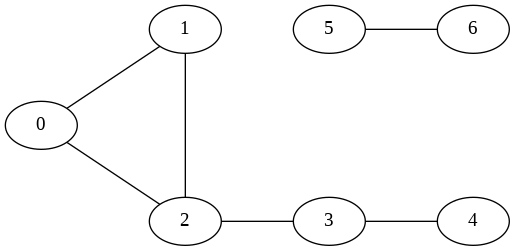
\includegraphics[width=0.49\columnwidth] {fig/chapter_advanced_graph/undirected_cyclic_graph.png}
    \caption{Undirected Cyclic Graph. $(0, 1, 2, 0)$ is a cycle}
    \label{fig:advanced_graph_ucg}
    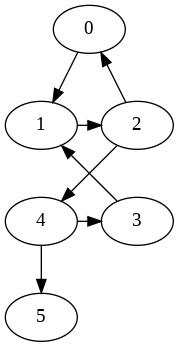
\includegraphics[width=0.49\columnwidth] {fig/chapter_advanced_graph/directed_cyclic_graph.png}
    \caption{Directed Cyclic Graph, $(0, 1, 2, 0)$ is a cycle.}
    \label{fig:cc_cycle}
\end{figure}
\paragraph{Problem Definition}
Detect cycles in both directed and undirected graph. Specifically, given a path with $k+1$ vertices, denoted as ${v_0, v_1, ..., v_k}$ in graph $G$:
\begin{enumerate}
    \item When $G$ is directed: a cycle is formed if $v_0=v_k$ and the path contains at least one edge.  For example,  there is a cycle ${0, 1, 2, 0}$ shown in the directed graph of Fig.~\ref{fig:cc_cycle}.
    \item When $G$ is undirected: the path forms a cycle only if $v_0=v_k$ and the path length is at least three (i.e., there are at least three distinct vertices within the path). For example, in the undirected graph of Fig.~\ref{fig:cc_cycle}, we couldn't say $(0, 2)$ is a cycle even though there is a path ${0, 2, 0}$, but the path ${0, 2, 1, 0}$ is as the path length $\geq 3$.
\end{enumerate}

\paragraph{DFS to Solve Cycle Detection} Recall the process of DFS graph search where a vertex has three possible states--white, gray, and black. A back edge appears while we reach to an adjacent vertex $v$ which is in gray state from current vertex $u$. 
If we connect $v$ back to its ancestor $u$, we find our cycle if the graph is directed.  
When the graph is undirected, we have discussed that it has only tree edge and back edge. 
Thus, we will use two states: visited and not visted. For edge $(u, v)$, we check two conditions:
\begin{enumerate}
  \item if $v$ is visited already. In Fig.~\ref{fig:advanced_graph_ucg}, when we are at $1$, we first visit $0$
  \item avoiding cycle of length one which is any existing edge within the graph. 
We can easily achieve this by tracking the predecessor $p$ of the exploring vertex during the search, and making sure the predecessor is not the same as the current vertex: $p\neq u$. %we need to distinguish between cycle of two nodes and cycle of more nodes. If this path includes two nodes as of $v_0, v_1, v_2$, when we are visiting $v_1$, the predecessor of $v_1$, which is $v_0$ will be the same as of $v_2$ which is a node with gray state. So, in addition to a normal DFS based cycle detection for the directed graph, we track the predecessor of the current visiting vertex. 
\end{enumerate}  

\paragraph{Cycle Detection for Directed Graph}  
We define a function \texttt{hasCycleDirected} with $g$ as the adjacent list of graph, $state$ as a list to track state for each vertex, and $s$ as the exploring vertex. The function returns a boolean value to indicate if there is a cycle or not. The function is essentially a DFS graph search along with an extra condition check on the back edge.  
\begin{lstlisting}[language=Python]
  def hasCycleDirected(g, s, state):
  state[s] = STATE.gray # first be visited
  for v in g[s]:
    if state[v] == STATE.white:
      if hasCycleDirected(g, v, state):
        print(f'Cycle found at node {v}.')
        return True
    elif state[v] == STATE.gray: # aback edge
      print(f'Cycle starts at node {v}.')
      return True
    else:
        pass
    state[s] = STATE.black # mark it as complete
    return False
\end{lstlisting}
Because a graph can be disconnected with multiple components, we run \texttt{hasCycleDirected} on each unvisited vertex within the graph in a main function.
\begin{lstlisting}[language=Python]
  def cycleDetectDirected(g):
  n = len(g)
  state = [STATE.white] * n
  for i in range(n):
    if state[i] == STATE.white:
      if hasCycleDirected(g, i, state):
        return True
  return False
\end{lstlisting}

\paragraph{Cycle Detection for Undirected Graph} First, we add another variable \texttt{p} to track the predecessor. 
$p$ will first be initialized to $-1$ because the root in the rooted search tree has no predecessor (or ancestor).  
 We can use the three coloring state as we did in directed graph, but it is a slight overkill. 
 In the implementation, we only use boolean value to mark its state:
\begin{lstlisting}[language=Python]
def hasCycleUndirected(g, s, p, visited):
  visited[s] = True
  for v in g[s]:
      if not visited[v]:
        if hasCycleUndirected(g, v, s, visited):
          print(f'Cycle found at node {v}.')
          return True
      else:
        if v != p: # both black and gray
          print(f'Cycle starts at node {v}.')
          return True
  return False
\end{lstlisting}
The main function:
\begin{lstlisting}[language=Python]
def cycleDetectUndirected(g):
  n = len(g)
  visited = [False] * n
  for i in range(n):
    if not visited[i]:
      if hasCycleUndirected(g, i, -1, visited):
        print(f'Cycle found at start node {i}.')
        return True

  return False
\end{lstlisting}
Please check the source code to try out the examples.

\begin{bclogo}[couleur = blue!30, arrondi=0.1,logo=\bccrayon,ombre=true]{How to find all cycles? {First, we need to enumerate all paths while searching in order to get all cycles. This requires us to retreat to less efficient search strategy: depth-first tree search. Second, for each path, we find where the cycle starts by comparing each $v_i$ with current vertex $u$: in directed graph, once $v_i==u$, the cycle is $v_i, v_{i+1}, ..., v_k, v_i$; in undirected graph, the cycle is found only if the length of $v_i, ..., v_k$ $\geq$ 3.}} 
\end{bclogo}

\section{Topological Sort}
\label{sec_topological_sort}
\paragraph{Problem Definition} In  a given Directed Acyclic Graph (DAG) $G=(V, E)$, \textit{topological sort/ordering} of is a linear ordering of the vertices $V$, such that for each edge $e \in E, e = (u, v)$, $u$ comes before $v$. If a vertex represents a task to be completed and each directed edge denotes the order between two tasks, then topological sort is a way of linearly ordering a number of tasks in a completable sequence. 
\begin{figure}[h]
    \centering
    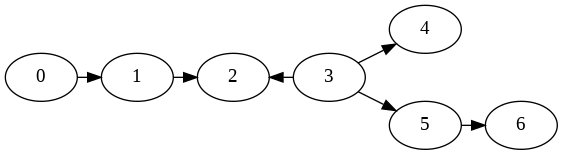
\includegraphics[width=0.7\columnwidth]{fig/chapter_advanced_graph/ts_2.png}
    \caption{DAG 1}
    \label{fig:dag_1}
\end{figure}

Every DAG has at least one topological ordering. For example, the topological ordering of Fig~\ref{fig:dag_1} can be \texttt{[0, 1, 3, (2, 4, 5), 6]}, where $(2, 4, 5)$  can be of any order, i.em., $(2, 4, 5), (2, 5, 4), (4, 2, 5), (4, 5, 2), (5, 2, 4), (5, 4, 2)$.

A topological ordering is only possible if there is no cycle existing in the graph. Thus, a cycle detection should be applied first when we are given a possible cyclic graph. 

% \begin{figure}[h]
%     \centering
%     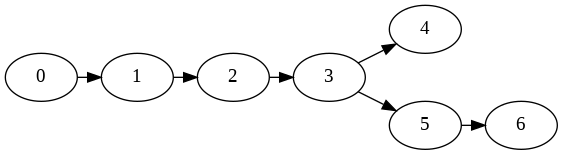
\includegraphics[width=0.7\columnwidth]{fig/chapter_advanced_graph/ts_1.png}
%     \caption{DAG 2}
%     \label{fig:dag_2}
% \end{figure}
\subsubsection{Kahn's algorithm (1962)} In topological sort, the first vertex is always ones with in-degree 0 (a vertex with no incoming edges). A naive algorithm is to decide the first node (with in-degree 0), add it in resulting order $S$, and remove all outgoing edges from this node. Repeat this process until: 
\begin{itemize}
    \item $V-S$ is empty, i.e., $|S|=|V|$, which indicates we found valid topological ordering.
    \item no node with 0 in-degree found in the remaining graph $G = (V-S, E^{'})$ where $E^{'}$ are the remaining edges from $E$ after the removal, i.e., $|S| < |V|$, indicating a cycle exists in $V-S$ and no valid answer exists.
\end{itemize}
For example, with the digraph in Fig.~\ref{fig:dag_1}, the process is:
\begin{lstlisting}[numbers=none]
S      Removed Edges
0, 3 are the in-degree 0 nodes
Add 0     (0, 1) 
1, 3 are the current in-degree 0 node
Add 1     (1, 2) 
3  is the only in-degree 0 node
Add 3     (3, 2), (3, 4), (3,5)
2, 4, 5 are the in-degree 0 nodes
Add 2
Add 4
Add 5    (5, 6)
6 is the only in-degree 0 node
Add 6
V-S empty, stop
\end{lstlisting}
In this process, we see that in some time 2, 4, 5 are no in-degree 0 nodes, that is why their orderings can be permutated, resulting multiple topological orderings. 

In implementation, instead of removing edges from the graph explicitly, a better option is to track $V-S$ with each vertex's in-degree: whenever a in-degree 0 vertex  $u$ is added into $S$,  $\forall v, u\rightarrow v$,  decrease the in-degree of $v$ by one. We also keep a queue of the all nodes with in-degree zero $Q$. Whenever a vertex in $V-S$ is detected with zero in-degree, add it into $Q$. Accumulatively, the cost of decreasing the in-degree for vertices in $V-S$ is $|E|$ as from the start to end,``all edges are removed.'' The cost of removing of vertex from $V-S$ is $|V|$ as all nodes are removed at the end.  With the initialization of the in-degree for vertices in $V-S$, we have a total of $O(2|E|+|V|)$, i.e., $O(|E|+|V|)$ as the time complexity. Python code:
\begin{lstlisting}[language=Python]
from collections import defaultdict
import heapq 
def kahns_topo_sort(g):
  S = []
  V_S =[(0, node) for node in range(len(g))] # initialize node with 0 as in-degree
  indegrees = defaultdict(int)
  # Step 1: count the in-degree
  for u in range(len(g)):
    indegrees[u] = 0
  for u in range(len(g)):
    for v in g[u]:
      indegrees[v]+= 1
  print(f'initial indegree : {indegrees}')
  V_S = [(indegree, node) for node, indegree in indegrees.items()]
  heapq.heapify(V_S)

  # Step 2: Kan's algorithm
  while len(V_S) > 0:
    indegree, first_node = V_S.pop(0)
    if indegree != 0: # cycle found, no topological ordering
      return None
    S.append(first_node)
    # Remove edges
    for v in g[first_node]:
      indegrees[v] -= 1
    # update V_S
    for idx, (indegree, node) in enumerate(V_S):
      if indegree != indegrees[node]:
        V_S[idx] = (indegrees[node], node)
    heapq.heapify(V_S)
  return S
\end{lstlisting}
Calling the function using graph in Fig.~\ref{fig:dag_1} gives result:
\begin{lstlisting}
initial indegree : defaultdict(<class 'int'>, {0: 0, 1: 1, 2: 2, 3: 0, 4: 1, 5: 1, 6: 1})
[0, 1, 3, 2, 4, 5, 6]
\end{lstlisting}

\subsubsection{Linear Topological Sort with Depth-first Graph Search} In depth-first graph search, if there is an edge $u\rightarrow v$, the recursive search from $v$ will always be completed ahead of the search of $u$.  With a simple reverse of the finishing ordering of vertices in depth-first graph search, the topological ordering takes $O(|E|+|V|)$ time. The time complexity equates to that of Kahn's algorithm, but this process is more efficient as it does not require the counting and updates of node in-degrees.  The whole process is exactly the same as Cycle Detection with additional complete ordering tracking.

First, the code of the DFS is:
\begin{lstlisting}[language=Python]
def dfs(g, s, colors, complete_orders):
  colors[s] = STATE.gray
  for v in g[s]:
    if colors[v] == STATE.white:
      if dfs(g, v, colors, complete_orders):
        return True
    elif colors[v] == STATE.gray: # a cycle appears
      print(f'Cycle found at node {v}.')
      return True
  colors[s] = STATE.black
  complete_orders.append(s)
  return False
\end{lstlisting}
Then main function is:
\begin{lstlisting}[language=Python]
def topo_sort(g):
  n = len(g)
  complete_orders = []
  colors = [STATE.white] * n
  for i in range(n): # run dfs on all the node
    if colors[i] == STATE.white:
      ans = dfs(g, i, colors, complete_orders)
      if not ans:    
        print('Cycle found, no topological ordering')
        return None 
  return complete_orders[::-1]
\end{lstlisting}
Call \texttt{topo\_sort} on the graph, we will have the sorted ordering as:
\begin{lstlisting}[language=Python]
[3, 5, 6, 4, 0, 1, 2]
\end{lstlisting}
which is another linear topological ordering.
\subsubsection{Example: Course Schedule (L210, m)}
There are a total of $n$ courses that you have to take. Some courses may have prerequisites, for example course 1 has to be taken before course 0, which is expressed as $[0, 1]$. Given the total number of courses and the prerequisite pairs, return the ordering of courses you should take to finish all courses. If it is impossible to finish, return an empty array. 

\paragraph{Analysis} Viewing a pair $[u, v]$ as an directed edge $v\rightarrow u$, we have a directed graph with $n$ vertices and we solve the ordering of courses as getting the topological sort of vertices in the resulting digraph. 

%%%%%%%%%%%%%%%%%%%%%%Connected Components%%%%%%%%%%%%%%%%%%%%%%%%%%%%%%%%%
\section{Connected Components}
\label{sec_connected_component}
\paragraph{Problem Definition}
In graph theory, a \textit{connected component}(or simply component) is defined as a subgraph where all vertices are mutually connected,  i.e., where there exists a path between any two vertices in it. A  graph $G = (V, E)$ is thus composed of separate connected components(sets) which are mutually exclusive and include all the vertices, .i.e., $V = V_0 \cup V_1 \cup ... \cup V_{m-1}, V_i \cap V_{j\neq i} = \emptyset $. A connected component algorithm should be able to cluster vertices of each single connected component. 
\begin{figure}[h]
    \centering
    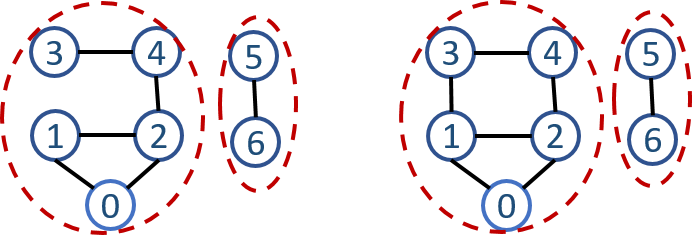
\includegraphics[width=0.6\columnwidth] {fig/undirected_cc_example.png}
    \caption{The connected components in undirected graph, each dashed read circle marks a connected component.}
    \label{fig:cc_undirected}
\end{figure}
% of an undirected graph in which any two vertices are connected to each other by paths, and which is connected to no additional vertices in the supergraph. 
For example, the undirected graph in Fig.~\ref{fig:cc_undirected} has two connected components: $\{0, 1, 2, 3, 4\}$ and $\{5, 6\}$. 

Given a  directed graph,
\begin{itemize}
    \item the term \textit{Strongly Connected Component (SCC)} or \textit{diconnected} is used to refer to the same definition-- where in a SCC any two vertices are reachable to each other by paths. In the leftest directed graph shown in  Fig.~\ref{fig:connected_components}, there is a total of five SCCs:  $\{0, 1, 2\}$, $\{3\}$,$\{4\}$, $\{5\}$, and $\{6\}$.  Vertex 5 and 6 is only connected in one way, resulting into two separate SCCs. 
    \item ignoring the direction of edges, a \textit{weakly connected component (WCC)} equates to a connected component in the resulting undirected graph.
\end{itemize} 
\begin{figure}[!ht]
    \centering
    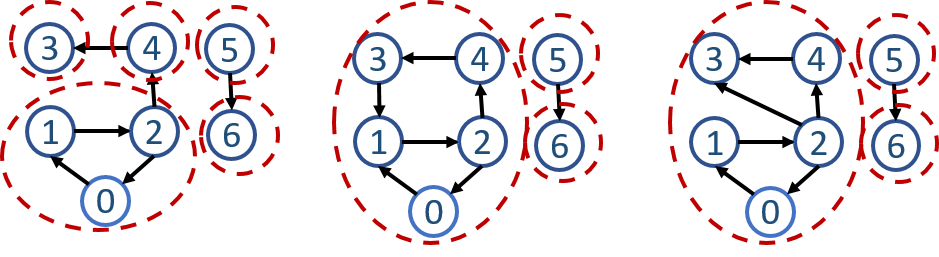
\includegraphics[width=0.8\columnwidth] {fig/directed_scc_example.png}
    \caption{The strongly connected components in directed graph, each dashed read circle marks a strongly connected component.}
    \label{fig:connected_components}
\end{figure}

\paragraph{Cycles and Strongly Connected Components} A directed graph is acyclic if and only it has no strongly connected subgraphs with more than one vertex. We call SCCs with at least two vertices nontrivial SCCs. Nontrial SCCs contains at least one directed cycle, and  more specifically, nontrivial SCCs is composed of a set of directed cycles as we have observed that there are two directed cycles in our above example and they share at least one common vertex. The shared common vertex act as ``transferring stop'' between these directed cycles thus they all compose to one component. Therefore, SCCs algorithms can be indirectly used to detect cycles. If there exists nontrivial SCC, directed graph contains cycles. 

\subsection{Connected Components Detection}
In general, there are two ways to detect connected components in an undirected graph: graph search and union-find, each suits different needs.
\paragraph{Graph Search and Search Tree} In  undirected graph $G$, executing a BFS or DFS starting at some vertex  $u$ will result in a rooted search tree. As the edges are undirected or bidirectional, all vertices in the search tree belong to the same connected component. To find all connected components, we simply loop through all vertices $V$, for each vertex $u$:
\begin{itemize}
    \item if $u$ is not visited yet, we start a new DFS/BFS. Mark all vertices along the traversal as the same component.
    \item otherwise, $u$ is already included in a previously found connected component, continue.
\end{itemize} 
The time complexity will be $O(|V|+|E|)$ and the space complexity will be $O(|V|)$. Since the code is trivial, we only demonstrate it in the notebook.
\subsubsection{Union Find}
We represent each connected component as a set. For the exemplary graph in Fig.~\ref{fig:cc_undirected}, we have two sets: ${0, 1, 2, 3, 4}$ and ${5, 6}$. Unlike the graph-search based approach, where the edges are visited in certain order,in union-find approach, the ordering of edges to be visited can be arbitrary. The algorithm using union-find is: 
\begin{itemize}
    \item Initialize in total $|V|$ sets, one for each vertex $V$.
    \item For each edge $(u, v)$ in $E$, \texttt{union} the two sets where vertex $u$ and $v$ previously belongs to.
\end{itemize}
Implementing it with Python:
\begin{lstlisting}[language=Python]
from collections import defaultdict
def connectedComponent(g):
  n = len(g)
  # initialize disjoint set
  ds = DisjointSet(n)

  for i in range(n):
    for j in g[i]: # for edge i<->j
      ds.union(i, j)
  return ds.get_num_sets(), ds.get_all_sets() 
\end{lstlisting}
How we implement the union-find data structure decides the complexity of this approach. For example, if we use linked list based structure, the complexity will be $O(|E|\times|V|)$ as we traversal $|V|$ edges and each step in worst case can take $O(|V|)$ to find the set that it belongs to. However, if path compression and union by rank is used for optimization, the time complexity could be lowered to $O(|E|\times \log|V|)$. 
\paragraph{Dynamic Graph} Since union-find has worse time complexity compared with graph search, then why do we care about it? The answer is: if we use graph search, whenever new edges and vertices are added to the graph, we have to rerun the graph search algorithm. Imagine that if we double $|V|$ and $E$, the worst time complexity will be $O(|V|\times (|V|+|E|)$, bringing up the complexity to polynomial of the number of edges. However, for each additional edge, union-find adds only a single merge operation to address the change, keeping the time complexity unchanged. 

In detail, we adapt the union-find structure dynamically. Set up a \texttt{dict} to track vertex and its index in the union find. Set \texttt{index=0}. When a new edge $(u, v)$ comes, union find includes:
\begin{itemize}
    \item check if $u$ and $v$ exists in \texttt{dict}. If not, (a) add a key-value into the node tracker, (b) append \texttt{index} into the list of vertex-set, (c) \texttt{index+=1}.
    \item \texttt{find} the sets where $u$ and $v$ belongs to. 
\end{itemize}
\paragraph{Implementation} Here we demonstrate how to implement a dynamic connected component detection algorithm. First, convert the graph representation from adjacent list to a list of edges:
\begin{lstlisting}[language=Python]
ug_edges = [(0, 1), (0, 2), (1, 2), (2, 4), (4, 3), (4, 3), (5, 6)]
\end{lstlisting}
Then, we implement a class \texttt{DynamicConnectedComponent} offering all functions needed.
\begin{lstlisting}[language=Python]
class DynamicConnectedComponent():
  def __init__(self):
    self.ds = DisjointSet(0)
    self.node_index= defaultdict(int)
    self.index_node = defaultdict(int)
    self.index = 0

  def add_edge(self, u, v):
    if u not in self.node_index:
      self.node_index[u], self.index_node[self.index] = self.index, u
      self.ds.p.append(self.index)
      self.ds.n += 1
      self.index += 1
      
    if v not in self.node_index:
      self.node_index[v], self.index_node[self.index] = self.index, v
      self.ds.p.append(self.index)
      self.ds.n += 1
      self.index += 1
    u, v = self.node_index[u], self.node_index[v]
    self.ds.union(u, v)
    return

  def get_num_sets(self):
    return self.ds.get_num_sets()

  def get_all_sets(self):
    sets = self.ds.get_all_sets()
    return {self.index_node[key] : set([self.index_node[i] for i in list(value)]) for key, value in sets.items()} 
\end{lstlisting}
Now, to find the connected components dynamically based on incoming edges, we can run:
\begin{lstlisting}[language=Python]
dcc = DynamicConnectedComponent()
for u, v in ug_edges: 
  dcc.add_edge(u, v)
dcc.get_num_sets(), dcc.get_all_sets()
\end{lstlisting}
The output is consistent with previous result, which is:
\begin{lstlisting}
(2, {3: {0, 1, 2, 3, 4}, 6: {5, 6}})
\end{lstlisting}
\subsubsection{Examples}
\begin{enumerate}
\item 547. Number of Provinces(medium)
    \item 128. Longest Consecutive Sequence (hard), union find solution: \url{https://leetcode.com/problems/longest-consecutive-sequence/discuss/1109808/Python-Clean-Union-Find-with-explanation}
\end{enumerate}
% Therefore, the additional cost for a newly added edge is constant, making the algorithm stable and linear all the time. Using the \texttt{DisjointSet} data structure implemented in Section \ref{}, our algorithm for running the above algorithm in a dynamic graph is implemented as:
% \begin{lstlisting}[language=Python]
% class UGraph():
%   def __init__(self, vertices, edges):
%     self.vertices = vertices
%     self.edges = edges
%     self.ds = DisjointSet(self.vertices)
%     self._init_connected_component()
%     print(f'The initial connected components are: {self.ds.set_item}')

%   def _init_connected_component(self):
%     for u, v in self.edges:
%       self.ds.union(u, v)
  
%   def add_edge(self, u, v):
%     # track nodes and make new set 
%     for node in [u, v]:
%       if node not in self.vertices:
%         self.vertices.add(node)
%       self.ds.make_set(node)

%     # track edges
%     if {u, v} not in self.edges:
%       self.edges.append({u, v})

%     # update ds
%     self.ds.union(u, v)
%     print(f'The  connected components are after adding edge ({u}, {v}) are: {self.ds.set_item}')
% \end{lstlisting}
\begin{bclogo}[couleur = blue!30, arrondi=0.1,logo=\bccrayon,ombre=true]{Implement WCC detection algorithm in directed graph? { }} 
\end{bclogo}
% \paragraph{Example: }

\subsection{Strongly Connected Components}
In graph theory, two nodes $u, v \in V$ are called strongly
connected iff $v$ is reachable from $u$ and
$u$ is reachable from $v$. If we contract each SCC into a single vertex, the resulting graph will be a DAG. Denoting the contracted DAG as $G^{SCC} = (V^{SCC}, E^{SCC})$, $V^{SCC}$ are vertices of SCCs and $E^{SCC}$ are defined as follows:

$(C_1, C_2)$ is an edge in $G^{SCC}$ iff $\exists u \in C_1, v \in C_2$. $(u, v)$ is an edge in $G$.

In other words, if there is an edge in $G$
from any node in $C_1$ to any node in $C_2$, there is an edge in $G^{SCC}$ from $C_1$ to $C_2$. 
\begin{figure}[!ht]
    \centering
    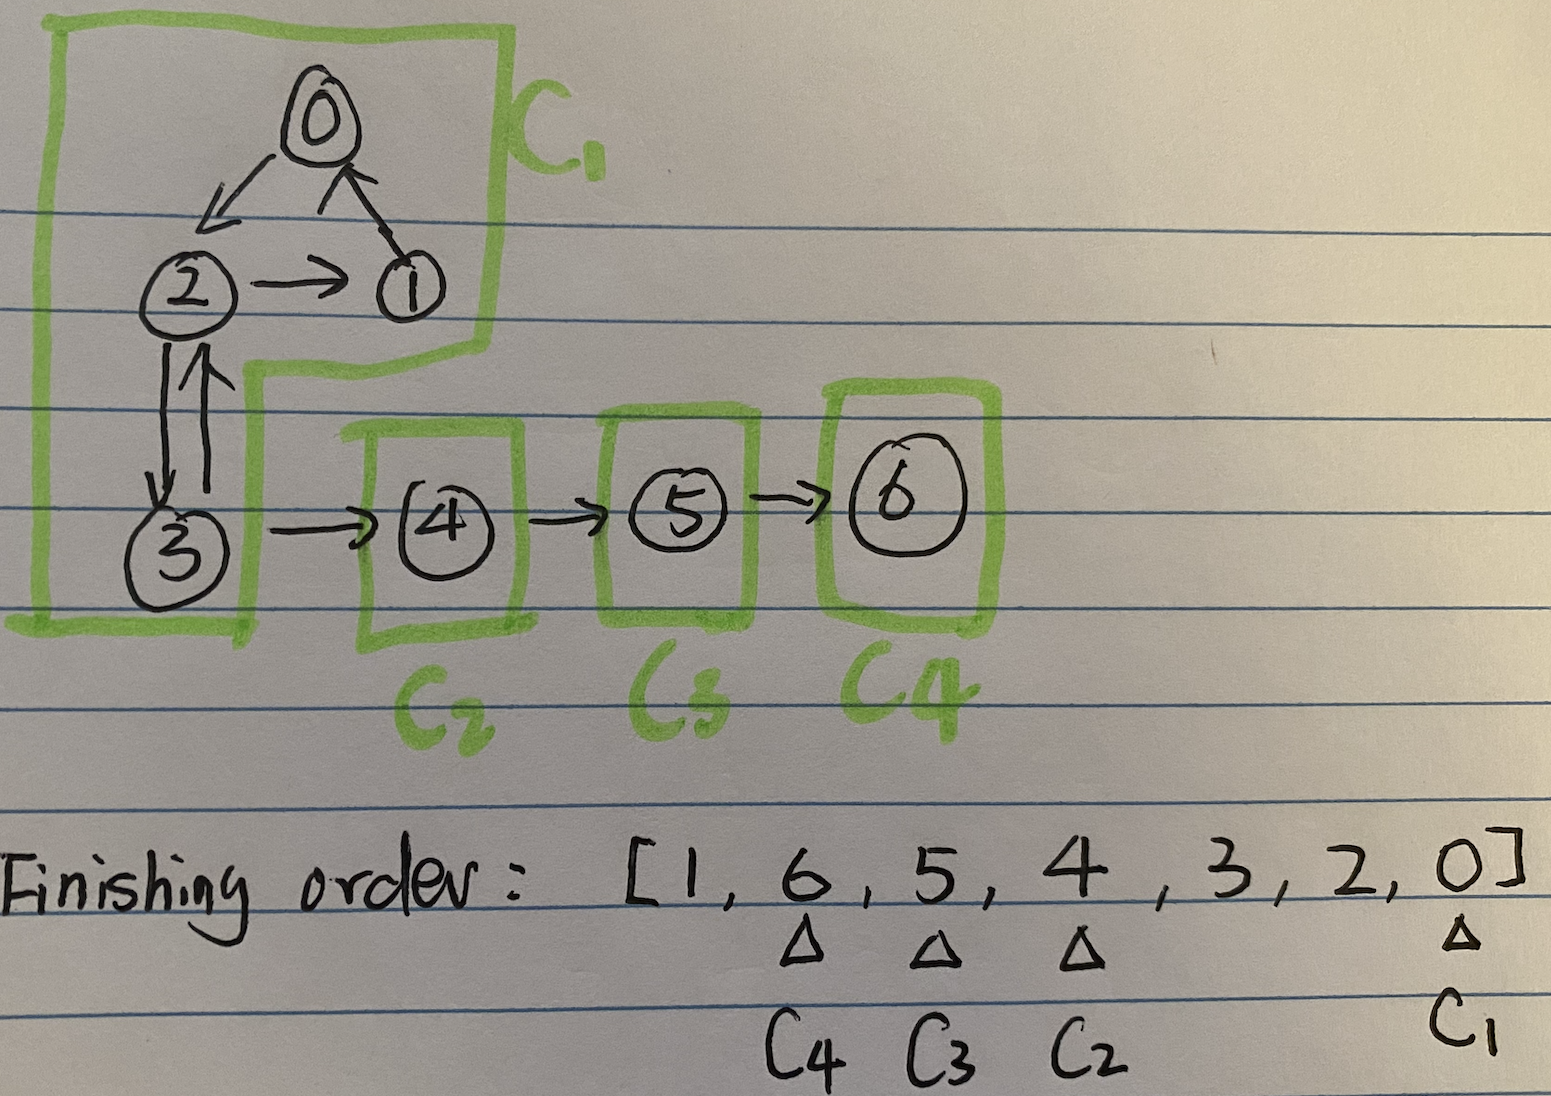
\includegraphics[width=0.85\columnwidth] {fig/chapter_advanced_graph/scc.png}
    \caption{A graph with four SCCs.}
    \label{fig:dfs_not_enough}
\end{figure}

\paragraph{Kosaraju's Algorithm} If we were to do a DFS in $G$, and  $C_1\rightarrow C_2$ is an edge in $G^{SCC}$, then at least one vertex in $C_1$ will finish after all vertices in $C_2$ being finished. If we first start with vertex $0$, the finishing order of of all vertices is [1, 6, 5, 4, 3, 2, 0]. $0$ finished later than $4$ from $C_2$, satisfying the claim. If we look purely at the last node from each SCC to turn dark, we get a topological sort of $G^{SCC}$ in reverse([1, \textcolor{red}{6}, \textcolor{red}{5}, \textcolor{red}{4}, 3, 2, \textcolor{red}{0}]), which is $[C_4, C_3, C_2, C_1]$. How to find the last node in each SCC? We can reverse the dfs finishing order, having [0, 2, 3, 4, 5, 6, 1]. 

If we reverse the order, we have [0, 2, 3, 4, 5, 6, 1]. What happens if we do another round of DFS on the given ordering? First, starting from 0 (last node), we can (1) reach to all vertices in $C_1$ as they are connected, (2) reach to vertices in $C_2$ if there exists no edge or edges only from $C_1$ to $C_2$ in between. If we can reverse the edges in between, then we can avoid (2) and still keeps (1). The way we do this is: reverse the direction of all edges in graph $G$. Run DFS on the reversed finishing ordering, then a SCC will include any vertex along the traversal that hasn's been put into a SCC yet. In our example, the process is:
\begin{lstlisting}[numbers=none]
0:  find {0, 1, 2, 3}
4: find {4}
5: find {5}
6: find {6}
\end{lstlisting}
We formalize Kosaraju's algorithm into three steps: 
\begin{enumerate}
\item Retrieve a reversed finishing order of vertices during DFS $L$. This step is similar to topological sort in an DAG.
\item Transpose the original graph $G$ to $G^T$ by reversing the directional of edges in $G$.
\item Run another DFS in $L_1$ ordering on $G^T$, any df-search tree starting from a vertex that hasn't been put into a SCC yet make up to another SCC. 
\end{enumerate}

\paragraph{Implementation} The main function \texttt{scc} calls two functions: \texttt{topo\_sort\_scc} and \texttt{reverse\_graph} to get $L$ and $G^T$. The topological ordering like function:
\begin{lstlisting}[language=Python]
# DFS traversal with reversed complete orders
def dfs(g, s, colors, complete_orders):
  colors[s] = STATE.gray
  for v in g[s]:
    if colors[v] == STATE.white:
      dfs(g, v, colors, complete_orders)
  colors[s] = STATE.black
  complete_orders.append(s)
  return
  
# topologically sort in terms of the last node of each scc
def topo_sort_scc(g):
  v = len(g)
  complete_orders = []
  colors = [STATE.white] * v
  for i in range(v): # run dfs on all the node
    if colors[i] == STATE.white:
      dfs(g,i, colors, complete_orders)
  return complete_orders[::-1]
\end{lstlisting}
The main scc is straightforward:
\begin{lstlisting}[language=Python]
# get conversed graph
def reverse_graph(g):
  rg = [[] for i in range(len(g))]
  for u in range(len(g)):
    for v in g[u]:
      rg[v].append(u)
  return rg
  
def scc(g):
  rg = reverse_graph(g)
  orders = topo_sort_scc(g)

  # track states
  colors = [STATE.white] * len(g)
  sccs = []

  # traverse the reversed graph
  for u in orders:
    if colors[u] != STATE.white:
      continue
    scc = []
    dfs(rg, u, colors, scc)
    sccs.append(scc)
  return sccs
\end{lstlisting}

\begin{bclogo}[couleur = blue!30, arrondi=0.1,logo=\bccrayon,ombre=true]{Try to take a look at Tarjans' algorithm for SCC} 
\end{bclogo}
\subsubsection{Examples}
\begin{enumerate}
    \item 1520. Maximum Number of Non-Overlapping Substrings (hard): set up 26 nodes for all letters. A node represents a substray from start to end.  Given a string abacdb, for a(0-2), add an edge between a -> to any other letter between start and end.Then we will have a directed graph. There is a scc (loop) between a and d, meaning a substring a has occurence of b and b substring has occurence of a, which is conflicting condition 2, so that they have to be combined. all results are sccs that are leaves in the contracted scc graph. We can think the scc graph is acyclic which is a forest. If we choose an internal node, we cant choose any of the leaves. Which making choosing the number of leaves maximum. Another solution is using two pointers: \url{https://zxi.mytechroad.com/blog/greedy/leetcode-1520-maximum-number-of-non-overlapping-substrings/}
\end{enumerate}
%%%%%%%%%%%%%%%%%%%%MST%%%%%%%%%%%%%%%%%%%%%%%%%%%%%%%%%%%%%%%
\section{Minimum Spanning Trees}
  \begin{figure}[!ht]
     \centering
     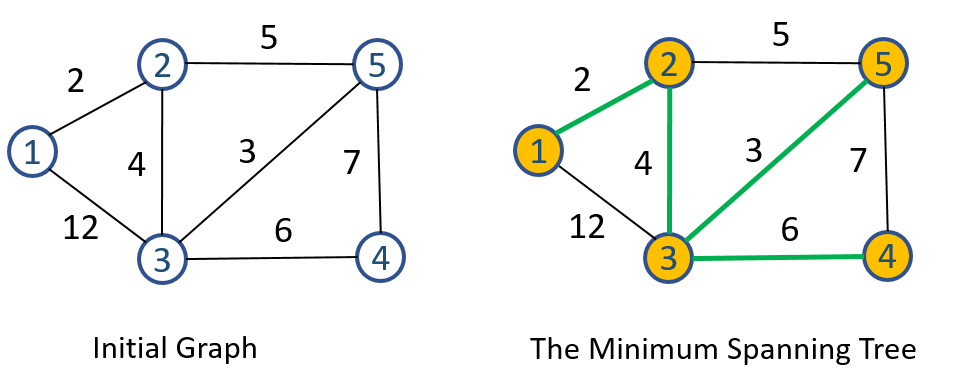
\includegraphics[width=0.99\columnwidth]{fig/mst_example.png}
     \caption{Example of minimum spanning tree in undirected graph, the green edges are edges of the tree, and the yellow filled vertices are vertices of MST (change this to a graph with multiple spanning tree, and highlight the one with the minimum ones.}
     \label{fig:prim_example}
 \end{figure}
\paragraph{Problem Definition} A \textit{spanning tree} in an undirected
graph $G=(V, E)$ is a set of edges, with
no cycles, that connects all vertices. There can exist many spanning trees in a graph. Given a weighted graph, we are particularly interested with  the \textit{minimum spanning tree (MST)}--a spanning tree with the least total edge cost.  

One example is shown in Fig.~\ref{fig:prim_example}.  This graph can represent a collection of houses, and possible wires that we can lay. How we lay wires
to connect all houses with the least total cost is equivalently a MST problem.

\paragraph{Spanning Tree}
To obtain a tree from a graph, the essence is to select edges iteratively until we have $|V|-1$ edges which form a tree connecting $V$. We have two general approaches:
\begin{itemize}
    \item Start with a forest consists of $|V|$ trees and contains only one node. We design a method to merge these trees into a final connected MST by selecting one edge at a time. This is the path taken by the Kruskal's algorithm.
    \item Start with a root node which can be any vertex selected from $G$, grow the tree by spanning to more nodes iteratively. In the process, we maintain two disjoint sets of vertices: one containing vertices that are in the growing spanning tree $S$ and the other to track all remaining vertices $V-S$.  This is the path taken by the Prim's algorithm.
\end{itemize}
We denote the edges in the growing as $A$. In this section, we explain two greedy algorithms to find MST.



\subsection{Kruskal's Algorithm}
  \begin{figure}[!ht]
     \centering
     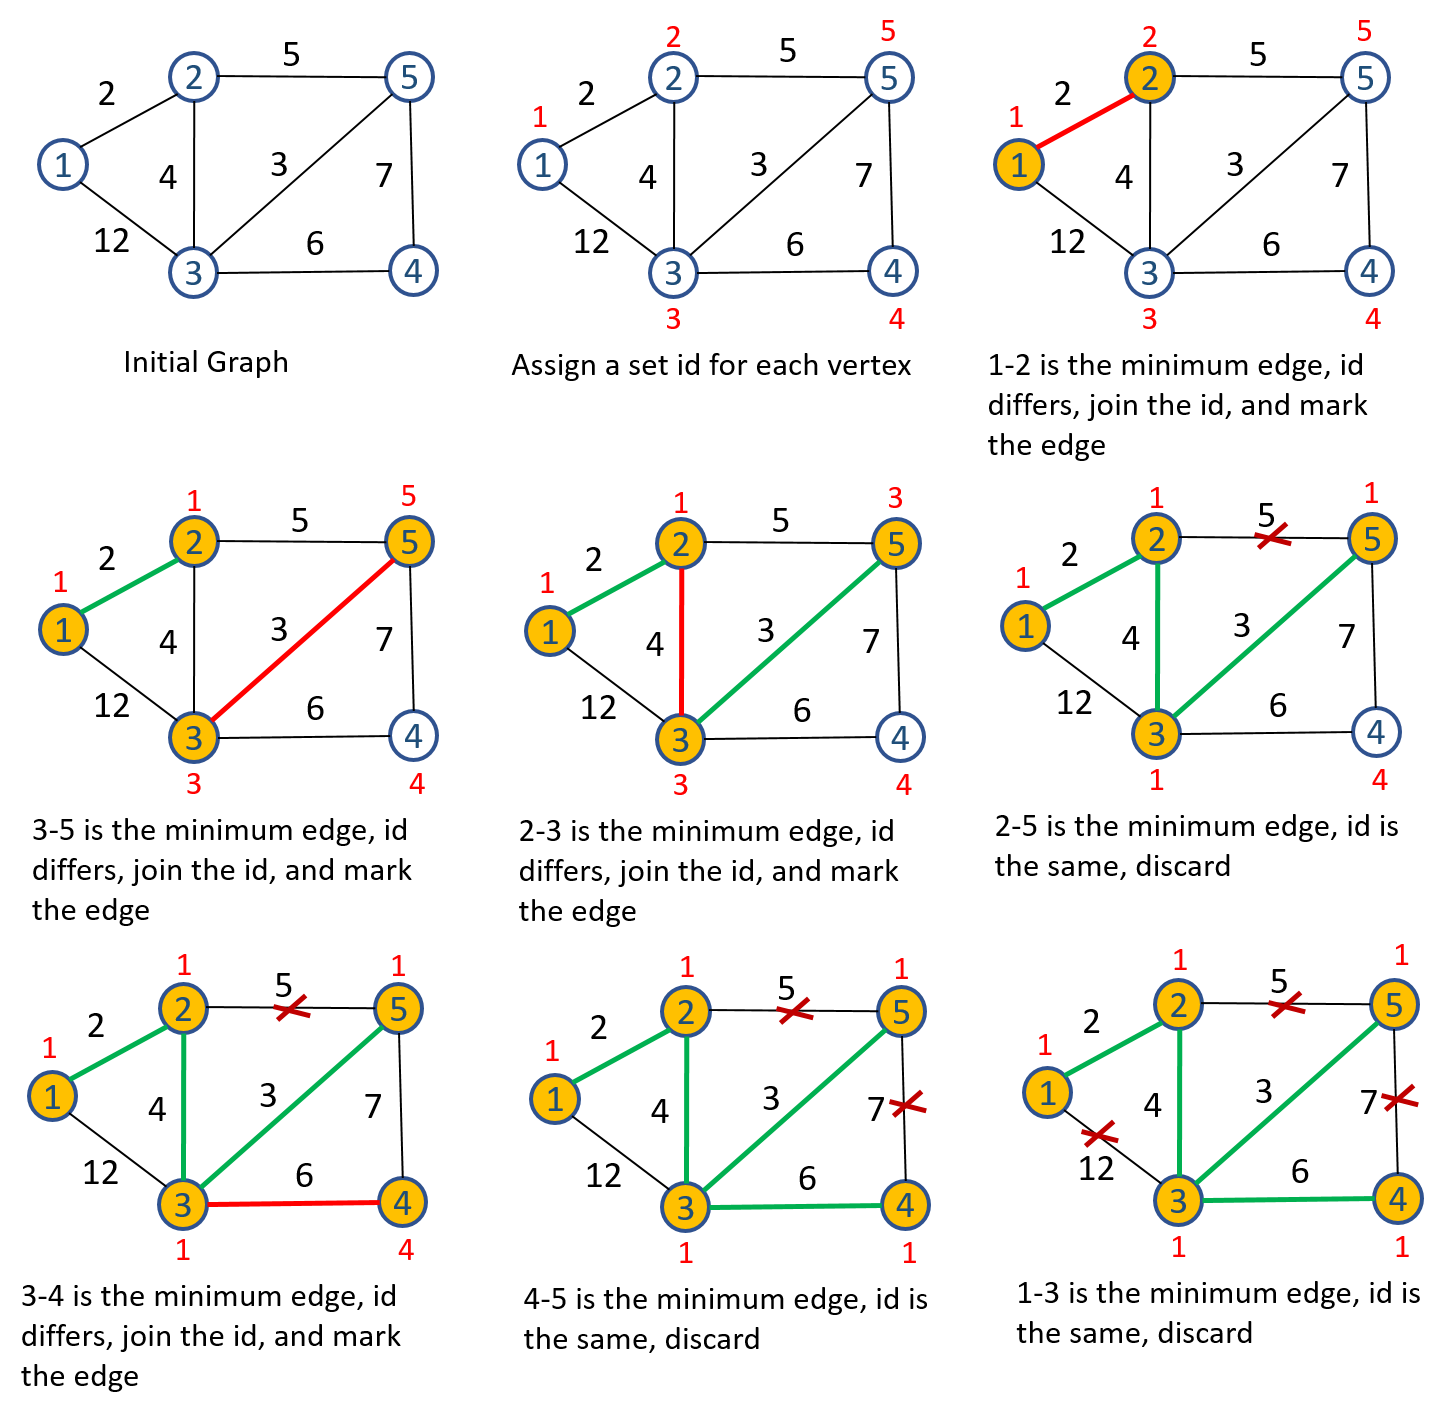
\includegraphics[width=0.99\columnwidth]{fig/mst_kruskal.png}
     \caption{The process of Kruskal's Algorithm}
     \label{fig:prim_kruskal}
 \end{figure}
Kruskal's algorithm starts with $|V|$ trees that each has only one node. The main process of the algorithm is to merge these trees into a single one by iterating through all edges.

\paragraph{Generate Spanning Tree with Union-Find} For each edge $(u, v)$:
\begin{itemize}
    \item if $u$ and $v$ belongs to the same tree, adding this edge will form a cycle, thus we discard this edge.
    \item otherwise, combine these two trees and add this edge into $A$.
\end{itemize}
This process will result in a single spanning tree. In implementation wise,  we can do this easily by using union-find data structure. A tree is a set. Adding one edge is to merge two sets/trees into a single one if they belong to different sets. 

\paragraph{Being Greedy with MST } 
 At each step $i$, we have $|E|-i$ edges to choose from. Applying the principle of greedy algorithm, maybe we can try to choose the edge with the minimum cost among $|E|-i$ options. That is to say, we iterate edges in increasing order of its weight in the process of generating a spanning tree. Doing so will ensure us to have the MST, and this algorithm is the so called Kruskal's algorithm. 

Fig.~\ref{fig:prim_kruskal} demonstrates the run of Kruskal's on the input undirected graph. Here, the edges are ordered increasingly, i.e., [(1,2), (3, 5), (2, 3), (2, 5), (3, 4), (4, 5), (1, 3)]. As initialization,  we assign a set id for each vertex that is marked in read and placed above its corresponding vertex. The process is:
\begin{lstlisting}[numbers=none]
edge     logic                                action
(1,2)    1's set_id 1 != 2's set_id 2       merge set 2 to set 1
(3,5)    3's set_id 3 != 5's set_id 5       merge set 5 to set 3
(2,3)    2's set_id 1 != 3's set_id 3       merge set 3 to set 1
(2,5)    2's set_id 1 == 5's set_id 1       continue
(3,4)    3's set_id 1 != 4's set_id 4       merge set 4 to set 1
(4,5)    4's set_id 1 == 5's set_id 1       continue
(1,3)    1's set_id 1 == 3's set_id 1       continue
\end{lstlisting}
This process produces edges $[(1,2), (3,5), (2,3), (3, 4)]$ as the edges of the final MST. We can have slightly better performance if we can stop iterating through edges once we have selected $|V|-1$ edges. The implementation is as simply as:
\begin{lstlisting}[language=Python]
from typing import Dict
def kruskal(g: Dict):
  # g is a dict with node: adjacent nodes
  vertices = [i for i in range(1, 1 + len(g))]
  vertices = g.keys()
  n  = len(vertices)
  ver_idx = {v: i for i, v in enumerate(vertices)}

  # initialize a disjoint set
  ds = DisjointSet(n)

  # sort all edges
  edges = []
  for u in vertices:
    for v, w in g[u]:
      if (v, u, w) not in edges:
        edges.append((u, v, w))
  edges.sort(key=lambda x: x[2])
  
  # main section
  A = []
  for u, v, w in edges:
    if ds.find(ver_idx[u]) != ds.find(ver_idx[v]):
      ds.union(ver_idx[u], ver_idx[v])
      print(f'{u} -> {v}: {w}')
      A.append((u, v, w))
  return A
\end{lstlisting}
For the exemplary graph, we denote an weighted edge as a (key, value) pair, where the value is a tuple of two with the first item being the other endpoint from the key vertex and the second item being the weight of the edge.  The graph will thus be represented by a dictionary, $\{$1:[(2, 2), (3, 12)], 2:[(1, 2), (3, 4), (5, 5)], 3:[(1, 12), (2, 4), (4, 6), (5, 3)], 4:[(3, 6),  (5, 7)], 5:[(2, 5), (3, 3), (4, 7)]$\}$. Running \texttt{kruskal(a)} will return the following edges:
\begin{lstlisting}[numbers=none]
[(1, 2, 2), (3, 5, 3), (2, 3, 4), (3, 4, 6)]
\end{lstlisting}
\paragraph{Complexity Analysis} The sorting takes $O(|E|\log|E|)$ big oh time. The cost of checking each edge's belonging set id and merging two trees into a single one is decided by the complexity of the disjoint set, it can range from $O(\log|V|)$ to $O(|V|)$. Therefore, we can conclude the time complexity will be  bounded by the sorting time, i.e., $O(|E|\log|E|)$. 
  

 \subsection{Prim's Algorithm}
%  \paragraph{Minimum Spanning Tree} With the above process, we are able to find an arbitrary spanning tree. To make sure this tree is the minimum among all, we have to make sure each time the edge we add is a \textit{safe edge}. A safe edge is  an edge that may be added to $A$ without violating the invariant that $A$ is a subset of some minimum spanning tree. 
  \begin{figure}[!ht]
     \centering
     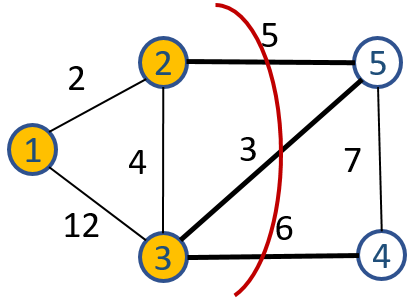
\includegraphics[width=0.45\columnwidth]{fig/graph_cut.png}
     \caption{A cut denoted with red curve partition V into \{1,2,3\} and \{4,5\}.}
     \label{fig:graph_cut}
 \end{figure}
  In graph theory, a \textit{cut} is a partition of $V$ into $S$ and $V-S$. For example, in Fig.~\ref{fig:graph_cut} a cut is marked by  red curve, removing three edges $(2, 5), (3, 5), (3, 4)$ partitions the set into two subgraph with subsets $\{1,2,3\}$ and $\{4,5\}$. A \textit{cross edge} $(u, v) \in E$ crosses the cut $(S, V-S)$ if  one of its endpoint is in $S$ and the other is in $V-S$. A \textit{light edge} is the minimum edge among all cross edges, such as edge $(3,5)$ is the light edge in our example. We say, a cut \textit{respects} a set of edges $A$ if no edge in $A$ crosses the cut, such as the marked cut in the example respects the set of edges $(1,2), (2, 3), (1, 3)$.
  
 Prim's algorithm starts with a randomly chosen root node and be put into a set $S$, leaving us with two sets of vertices, $S$ and $V-S$. Next, it iteratively grows the  partial and connected MST by adding an edge from the cross edges between the cut of $(S, V-S)$. Prim's algorithm is greedy in the sense that it chooses a  light edge  among its options to form the final MST.  \textcolor{red}{This process simulates the uniform-cost search which compose the Dijkstra's shortest path algorithm.} 
 
  \begin{figure}[!ht]
     \centering
     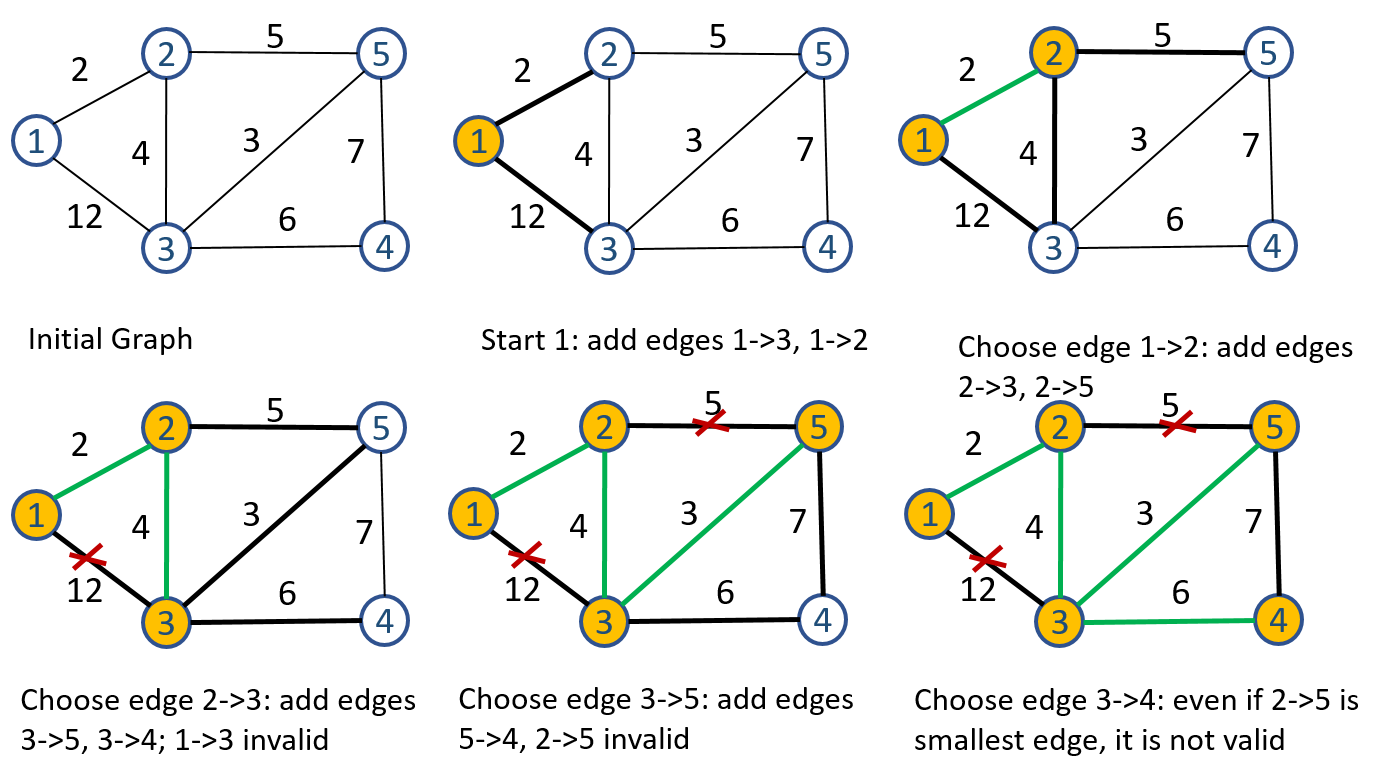
\includegraphics[width=0.99\columnwidth]{fig/mst_prim_2.png}
     \caption{Prim's Algorithm, at each step, we manage the cross edges.}
     \label{fig:prim_1}
 \end{figure}
 Fig.~\ref{fig:prim_1} demonstrates the process of Prim's algorithm. We start from vertex $1$. with the set $A$, $S$, $V-S$, the cross edges at each step are denoted as $CE$, and a decision valid if it does not form a cycle within $A$, we list the process as:
 \begin{lstlisting}[numbers=none]
 A                     S       V-S      CE          light edge
                       1     2,3,4,5  (1,2), (1,3)     (1,2)
(1,2)                 1,2     3,4,5 (1,3),(2,3),(2,5)  (2,3)
(1,2),(2,3)          1,2,3    4,5   (3,4),(3,5),(2,5)  (3,5) 
(1,2),(2,3),(3,5)   1,2,3,5    4   (3,4),(5,4)         (3,4) 
(1,2),(2,3),(3,5),(3,4) 1,2,3,4,5
\end{lstlisting}
 
\subsubsection{Implementation} One key step is to track all valid cross edges and be able to select the minimum edge from the set. Naturally, we use priority queue \texttt{pq}. \texttt{pq} can be implemented in two ways:
\begin{itemize}
    \item \textbf{Priority Queue by Edges}--Considering the set $S$ as a frontier set, \texttt{pq} maintains all edges expanded from the frontier set.
    \item \textbf{Priority Queue by Vertices}--\texttt{pq} maintains the minimum cross edge cost between vertices in $S$ to the current vertex which is in $|V-S|$. This is an optimization over the first approach as it reduces multiple cross edges between $S$ and current vertex $v$ into a single cost -- the minimum. 
    %We can represent the cost update for $v$ as $\min_u c(u, v), u \in S, (u, v) \in E$.  
\end{itemize}
\paragraph{Priority Queue by Edges} For example shown in Fig.~\ref{fig:prim_1}, at first, the frontier set has only $1$, then we have edges $(1,2), (1,3)$ in \texttt{pq}. Once edge $(1,2)$ is popped out as it has the smallest weight, we explore all outgoing edges of vertex 2 to nodes in $V-S$, adding $(2,3), (2,5)$ in \texttt{pq}, resulting $pq=(2,3),(2,5),(1,3)$. Then we pop out edge $(2,3)$, and explore outgoing edges of vertex 3 and add $(3,4),(3,5)$ into \texttt{pq}, with $pq=(2,5),(1,3),(3,4),(3,5)$. At this moment, we can see that edge $(1,3)$ is no longer a cross edge. Therefore, whenever we are about to add the light edge into the expanding tree, we check if both of its endpoints are in set $S$ already. If true, we skip this edge and use the next valid light edge. Repeat this process will get us the set of edges $A$ forming a MST. The Python code is as:
\begin{lstlisting}[language=Python]
import queue

def _get_light_edge(pq, S):
  while pq:
    # Pick the light edge
    w, u, v = pq.get()
    # Filter out non-cross edge
    if v not in S:
      S.add(v)
      return (u, v, w)
  return None
  
def prim(g):
  cur = 1
  n = len(g.items())
  S = {cur} #spanning tree set
  pq = queue.PriorityQueue()
  A = []
  
  while len(S) < n:
    # Expand edges for the exploring vertex
    for v, w in g[cur]:
      if v not in S:
        pq.put((w, cur, v))

    le = _get_light_edge(pq, S)
    if le:
      A.append(le)
      cur = le[1] #set the exploring vertex
    else:
      print(f'Graph {g} is not connected.')
      break
  return A
\end{lstlisting}
In line 24, we use a 3 item tuple representing the edge cost, the first endpoint in the set $S$ and the second endpoint in $V-S$ to align with the fact that the \texttt{PriorityQueue()} uses the first item of a tuple as the key for sorting. The \texttt{while} loop is similar to our breath-first-search and can be terminated in the following two conditions:
\begin{itemize}
    \item when the set $S$ is as large as the set $V$ by checking the size of set $S$
    \item when we can not find a light edge which happens when the graph is not connected.
\end{itemize}
Call \texttt{prim(a)} will return us the following $A$:
\begin{lstlisting}[numbers=none]
[(1, 2, 2), (2, 3, 4), (3, 5, 3), (3, 4, 6)]
\end{lstlisting}
\paragraph{Complexity Analysis} The main cost of this implementation is on the priority queue, which has a maximum of $|E|$ items. In the worst case we have to enqueue and dequeue all edges, making the complexity as $O(|E|\log|E|)$. In a graph, generally, $E < V^2$, the complexity become $O(|E|\log V)$.
\paragraph{Priority Queue by Vertices}
Instead of tracking cross edges in the priority queue explicitly, we reduce all cross edges that reaches to a vertex in $V-S$ into the smallest cost and a predecessor which is to track the node in $S$ that resulted in the smallest cost, saving us some additional space and time in the queue operations. 
% \begin{itemize}
%     \item If a vertex $v$ in $V-S$ is not connected to any vertex in $S$, it has a $\infty$ cost.
%     \item If this vertex $v$ is connected to one vertex $u$ in $S$ through edge $(u, v)$ which has an edge cost $w$, this vertex will have a cost $w$.
%     \item If this vertex $v$ is connected to multiple vertices in $S$, keep the smallest edge cost as its cost.
% \end{itemize}

  \begin{figure}[!ht]
     \centering
     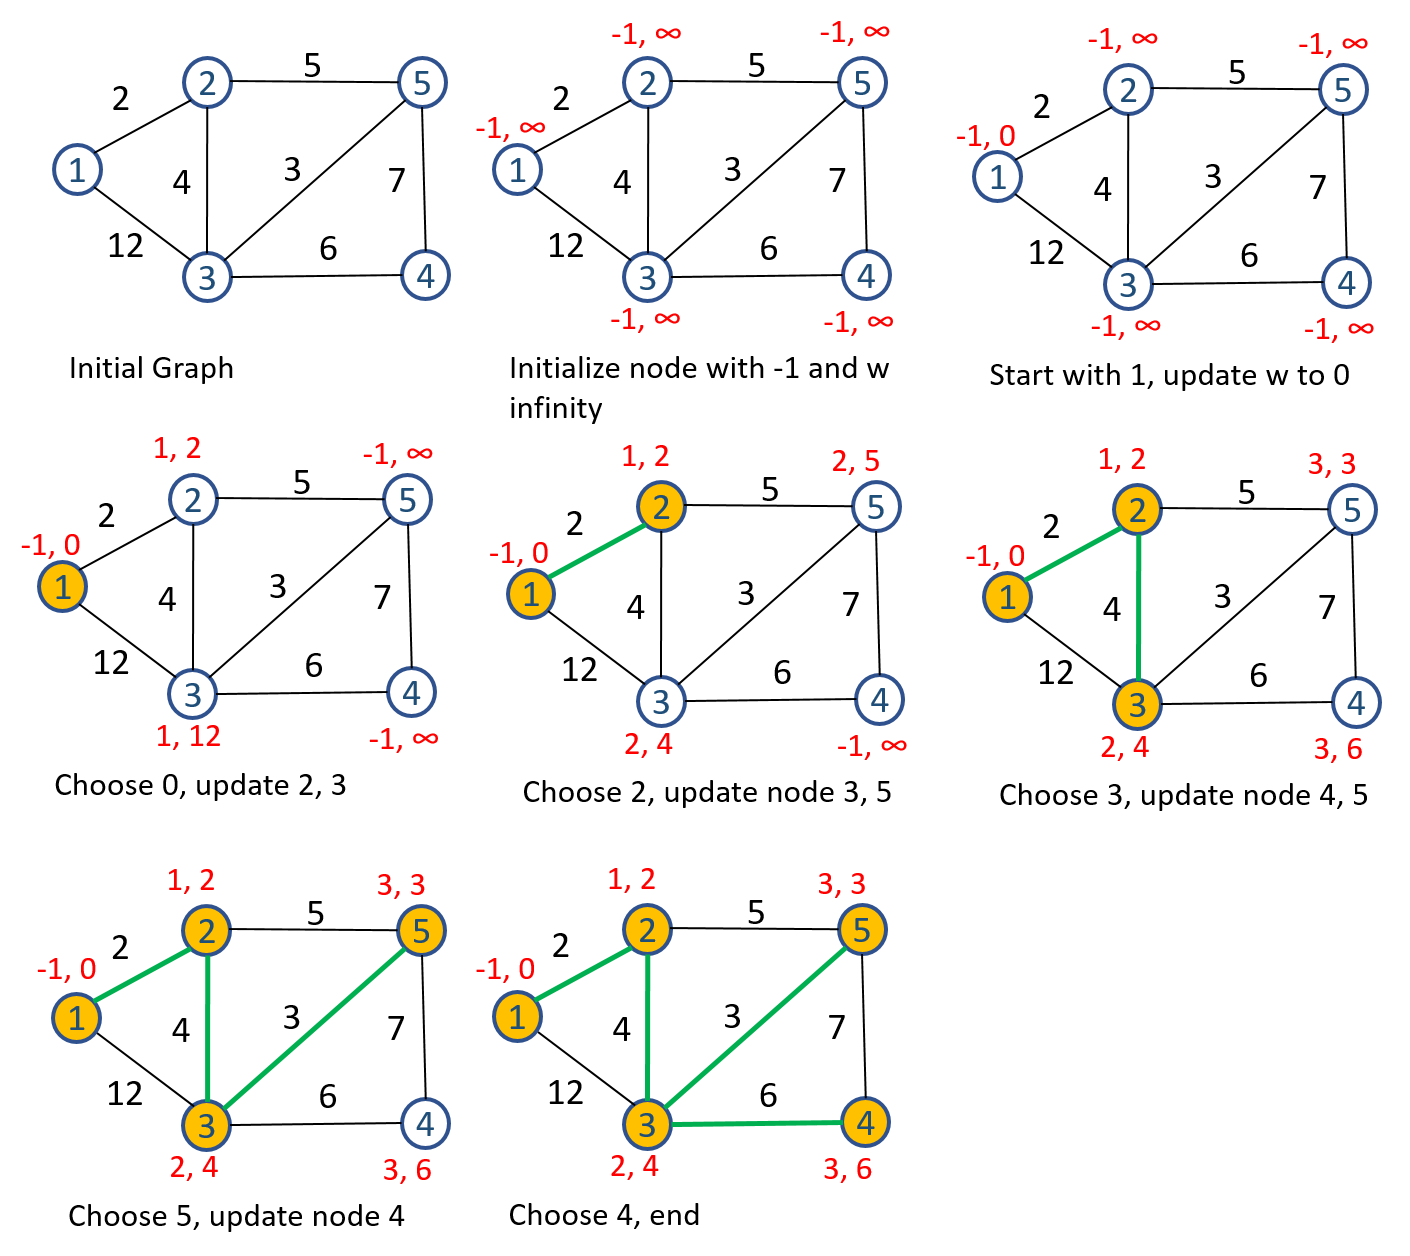
\includegraphics[width=0.99\columnwidth]{fig/mst_prim_1.png}
     \caption{Prim's Algorithm}
     \label{fig:prim_2}
 \end{figure}
 As shown in Fig.~\ref{fig:prim_2}, we first initialize a priority queue with $|V|$ items, each has a task id same as the vertex id, a predecessor vertex $p=-1$, and a cost initialized with $\infty$. We start by pointing vertex $1$ as the root node, setting $S={1}$ and modify the task 1's cost to 0 and points its predecessor to itself. Then, we repeatedly pop out the vertex in the queue that has the smallest weight, along with the predecessor of this node, we are choosing the light edge. With this chosen node, we are able to reach out to adjacent nodes that are still in $V-S$ and see if we are able to find an even ``lighter'' edge.  Applying this process on the given example:
 \begin{enumerate}
     \item First, we  have the start vertex 1 with the smallest cost, pop it out, and explore edges $(1,2), (1, 3)$, resulting in (a) modifying task 2 and 3's cost to 2 and 12, respectively and (b) set 2 and 3's predecessor to 1.
     \item Pop out vertex 2, explore edges $(2,3), (2,5)$, resulting in (a) modifying task 3 and 5's cost to 4 and 5, respectively and (b) set 3 and 5's predecessor to 2.
     \item Pop out vertex 3, explore edges $(3, 5), (3,4)$, resulting in (a) modifying task 5 and 4's cost to 3 and 6, respectively and (b) set 3 and 5's predecessor to 3.
     \item Pop out vertex 5, explore edges $(5, 4)$: since the new cross edge $(5,4)$ has larger cost compared with previous reduced cross edge to reach to vertex 4, the vertex 4 in the queue is not modified. 
     \item Pop out vertex 4, no more new edges to expand, terminate the program. 
 \end{enumerate}
 This process results in the exactly same MST compared with the implementation by edges. However, it adds additional challenges into the implementation of the priority queue: We have to modify an enqueued item's record during the life cycle of the queue. In the Python implementation, we use the our customized \texttt{PriorityQueue()} in Section.~\ref{}(also included in the notebook). The main process of the algorithm is:
 \begin{lstlisting}[language=Python]
def prim2(g):  
  n = len(g.items())
  pq = PriorityQueue()
  S = {}
  A = []
  # Initialization
  for i in range(n):
    pq.add_task(task=i+1, priority=float('inf'), info=None) # task: vertex, priority: edge cost, info: predecessor vertex
  
  S = {1}
  pq.add_task(1, 0, info=1)

  while len(S) < n:
    u, p, w = pq.pop_task()
    if w == float('inf'):
      print(f'Graph {g} is not connected.')
      break
    A.append((p, u, w))
    S.add(u)
    for v, w in g[u]:
      if v not in S and  w < pq.entry_finder[v][0]:
        pq.add_task(v, w, u)
  
  return A
 \end{lstlisting}
 Calling function \texttt{prim2(a)} will output the following $A$:
 \begin{lstlisting}[language=Python]
 [(1, 1, 0), (1, 2, 2), (2, 3, 4), (3, 5, 3), (3, 4, 6)]
 \end{lstlisting}
 
 \subsubsection{Examples}
 \begin{enumerate}
     \item 1584. Min Cost to Connect All Points (medium)
     \item 1579. Remove Max Number of Edges to Keep Graph Fully Traversable (hard)
 \end{enumerate}

\begin{bclogo}[couleur = blue!30, arrondi=0.1,logo=\bccrayon,ombre=true]{Try to prove the correctness of Kruskal's Algorithm.} 
\end{bclogo}


 
%%%%%%%%%%%%%%%%%%%%Shortest-Paths Algorithms%%%%%%%%%%%%%%%%%%%%%%%%%%%%
\section{Shortest-Paths Algorithms}
\label{sec_single_source_shortest_paths}
\paragraph{Problem Definition} Given a weighted, directed graph $G=(V, E)$, with weight function $w:E\rightarrow R$ that maps edges to real-valued weights, the weight of a path $p = (v_0, v_1, ..., v_k)$ is the summation over its constituent edge weights, denoted as $w(p)$: 
\begin{equation}
    w(p)=\sum_{i=1}^{k} w(v_{i-1}, v_i)
\end{equation}
\textit{The shortest path} problem  between $v_i$ and $v_j$ is to find the shortest path weight $\sigma(v_i, v_j)$ along with the shortest path $p$. 
\begin{equation}
\sigma(v_i, v_j) = \left\{ 
\begin{array}{ll}
\min\{w(p):v_i\xrightarrow{\text{p}} v_j\} & \mbox{if there is a path from  } v_i \mbox{ to } v_j \\
\infty &\mbox{otherwise}
\end{array}
\right.
\end{equation} 
\begin{figure}[!ht]
    \centering
    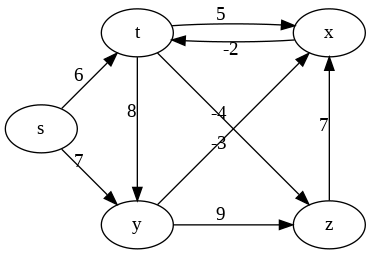
\includegraphics[width=0.6\columnwidth]{fig/directed_graph_negative.png}
    \caption{A weighted and directed graph.}
    \label{fig:sp_udg}
\end{figure}
For example, for the graph shown in Fig.~\ref{fig:sp_udg}, the shortest-path weight and its corresponding shortest-path between $s$ to any other vertex in $V$ is listed as:
\begin{lstlisting}[numbers=none]
(source, target)   shortest-path weight   shortest path
(s, s)                 0                      s
(s, y)                 7                   (s, y)
(s, x)                 4                   (s, y, x)
(s, t)                 2                   (s, y, x, t)
(s, z)                -2                  (s, y, x, t, z)
\end{lstlisting}

\paragraph{Variants of Shortest-path Problems} Generally, there exists a few variants of shortest path problems:
\begin{enumerate}
    \item \textit{Single-source shortest-path:} Find a shortest path from a given source $s$ vertex to each vertex $v \in V$.
    \item \textit{Single-target shortest-path:} Find a shortest path to a given target $t$ from each vertex  $v \in V$. By reversing the direction of each edge in the graph, we can reduce this problem to a single-source shortest-path problem.
    \item \textit{Single-pair shortest-path problem:} Find a shortest path from $u$ to $v$ for given vertices $u$ and $v$. If we solve the single-source problem with source vertex $u$, we solve this problem too. %Moreover, all known algorithms for this problem have the same worst-case asympototic running time as the best single-source algorithms.
    \item \textit{All-pairs shortest-path problem:} Find a shortest path from $u$ to $v$ for every pair of vertices $u$ and $v$ in $V$ if there exists one. Although we can solve this problem by running a single-source algorithm once for each vertex, we usually can solve it faster with algorithms addressed in Section (Sec.~\ref{sec_all_pairs_shortest_paths}).
\end{enumerate}

% As we can see, the single-source shortest-path problem is essential to any other mutants, we first discuss the algorithm design and analysis for this type. With its solution at hand, we further address the all-pairs shortest path problem. 

\subsection{Algorithm Design}
\label{chapter_advanced_graph_sec_algorithm_design}
In this section, we discuss the shortest path problem, and analyze it by using both graph theory and  the fundamental algorithm design principle--Dynamic Programming. 
\paragraph{Shortest path and Cycle} From our experience in Combinatorial Search, we have to detect cycles within a path in the graph-based tree search to avoid being stuck in infinite recursion. So, how will cycle affect the detection of shortest paths? For example, in Fig.~\ref{fig:sp_udg}, a path $p=(s, t, x, t)$ contains the cycle $(t, x, t)$.  Because the cycle has a positive path weight $5+(-2)$, the path $(s, t)$ remains smaller than the path that comes with the cycle. However, if we switch the weight of edge $(t, x)$ with that of $(x, t)$, then the same cycle $(t, x, t)$ will have negative path weight $(-5)+2$, repeating the cycle within the path infinitely we will have a cost of $-\infty$. Therefore, for a graph where the weights can be both negative and positive, one requirement posed on the single-source shortest-path algorithm, recursive or iterative, is to detect the negative-weight cycle that is reachable from the source. Once we get rid of all negative-weight cycles, the remaining of the algorithm can focus on only shortest-paths of at most $|V|-1$ edges, and the resulting shortest-paths will not contain neither negative- nor positive-weight cycles.

\subsubsection{Exponential Naive Solution}
% Therefore, when we are designing shortest-path algorithms for our given problems, it is important to address questions:
% \begin{enumerate}
%     \item Does the graph have a weight function that is non-negative? If true, we can use \textbf{Dijkstra's algorithm} detailed in Subsection~\ref{subsec_dijkstra}.
%     \item If not, is the graph acyclic? If it is acyclic, then a negative-weight cycle will never exist in the graph. We solve our problems with \textbf{Single-source shortest paths in directed acyclic graphs} in Subsection~\ref{subsec_general_shortest_path}. 
%     \item If the graph is potentially cyclic, and potentially end up with negative-weight cycle, we go for \textbf{Bellman-Ford Algorithm} (subsection~\ref{subsec_bellman_ford}) for answer. 
% \end{enumerate}
Assume the given graph has no negative-weight cycle, a naive solution to obtain the shortest path and its weight is simply through a tree-search which starts from a source vertex $s$ and enumerates all possible paths between $s$ to any other vertex in $V$. The search tree will have a maximum height of $|V|-1$, making the time complexity of this naive solution to be $O(b^{|V|})$, where $b$ is the maximum branch of a vertex. Recall the path enumeration in Search Strategies, we implement this solution as:
\begin{lstlisting}[language=Python]
def all_paths(g, s, path, cost, ans):
  ans.append({'path': path[::], 'cost': cost})
  for v, w in g[s]:
    # Avoid cycle
    if v in path:
      continue
    path.append(v)
    cost += w
    all_paths(g, v, path, cost, ans)
    cost -= w
    path.pop()
\end{lstlisting}
To obtain all possible paths, we call the function \texttt{all\_paths()} with the following code:
\begin{lstlisting}[language=Python]
g = {
    't':[('x', 5), ('y', 8), ('z', -4)],
    'x':[('t',-2)],
    'y':[('x',-3), ('z',9)],
    'z':[('x',7)],
    's':[('t', 6), ('y', 7)],   
}
ans = []
all_paths(g, 's', ['s'], 0, ans)
\end{lstlisting}
\begin{figure}[!ht]
    \centering
    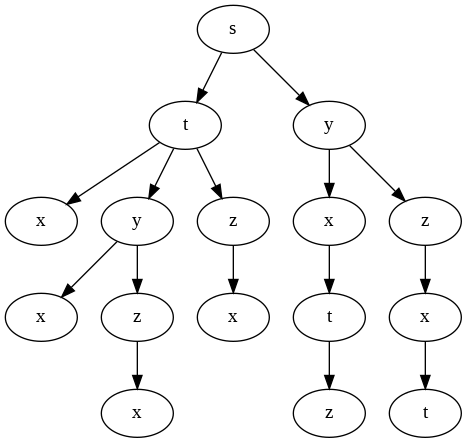
\includegraphics[width=0.6\columnwidth, height=8cm]{fig/all_paths_demo.png}
    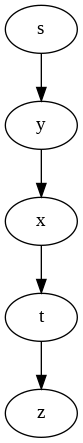
\includegraphics[width=0.1\columnwidth, height=8cm]{fig/shortest_path_demo.png}
        \caption{All paths from source vertex $s$ for graph in Fig.~\ref{fig:sp_udg} and its shortest paths.}
    \label{fig:sp_udg_all_paths}
\end{figure}
\paragraph{Shortest-paths Tree} We visualize all paths in \texttt{ans} in a tree structure shown in Fig.~\ref{fig:sp_udg_all_paths}. We can easily extract the shortest paths between $s$ to any other vertex from this result, which is shown on the right side of Fig.~\ref{fig:sp_udg_all_paths}. All possible paths starting from source vertex can be viewed as a tree, and the shortest paths from source to all other vertices within the graph will be a subtree of the former tree structure, known as the \textit{shortest-paths tree}. Formally, a shortest-paths tree rooted at $s$ is a directed subgraph $G^{'}=(V^{'}, E^{'})$, where $V^{'}\in V$ and $E^{'}\in E$, such that
\begin{enumerate}
    \item $V^{'}$ is the set of vertices reachable from $s$ in $G$,
    \item for each $v \in V^{'}$, the unique simple path from $s$ to $v$ in $G^{'}$ is a shortest path from $s$ to $v$ in $G$.
\end{enumerate}
\paragraph{Predecessor Rule}
The shortest-paths tree makes it possible for us to track shortest paths with the predecessor rule: Given a graph $G=(V,E)$, and in the single-source shortest path problem, we maintain for each vertex $v\in V$ a predecessor $\pi$ that is either another vertex or empty as for the root node. The shortest-paths between $s$ and another vertex $v$ can be obtained by iterating the chained predecessors starting from $v$ and all the way backward to the source $s$. To summarize, each vertex $v$ in the graph stores
two values, $d(v)$ and $\pi(v)$ , which (inductively) describe a tentative shortest path from $s$ to $v$.

% If there is negative-weight cycle, the above naive solution would fail us to detect that cycle
\subsubsection{Optimization}
As we see, shortest path problem is a truly combinatorial optimization problem, making them the best demonstration examples of the algorithm design principles--Dynamic Programming and Greedy Algorithm. On the other hand, depending on the characteristics of targeting graph, either they are dense or spares, directed acyclic graph (DAG) or not DAG, we can further optimize the efficiency besides of the design principle. However, in this chapter, we focus on the gist: \textit{how to solve all-pair shortest path problems with dynamic programming?}

% in this section, we will recall the properties of Dynamic Programming in the context of solving the shortest path problem: overlapping subproblems and optimal substructures. 
% \begin{figure}[!ht]
%     \centering
%     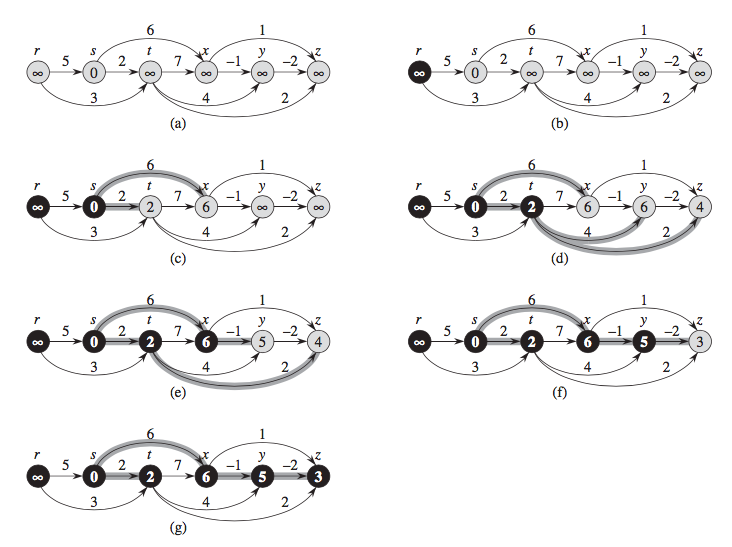
\includegraphics[width=0.95\columnwidth]{fig/shortest_path_property_1.png}
%     \caption{Flattening graph for better observation}
%     \label{fig:shortest_path_pro_1}
% \end{figure}

First, we use an adjacency matrix to represent our weight matrix $W$ of size $|V|\times |V|$. In the process, we track shortest-path weight estimate $D$ and additionally the predecessor $\Pi$. Both $D$ and $\Pi$ are of same size as $W$. $w_{ij}$ indicates the weight of each edge with startpoint $i$ and endpoint $j$, 
\begin{equation}
     W{(i, j)} = \left\{ 
    \begin{array}{lll}
   0 & \mbox{if   } i=j  \\
   w_{ij} & \mbox{if $i\ne j$, and  $(i, j)\in E$ } \\
    \infty & \mbox{if $i\ne j$, and  $(i, j)\notin E$ }
    \end{array}
    \right.
\end{equation}
With this definition, we show a naive directed graph in Fig.~\ref{fig:naive_graph} along with its $W$. 
\begin{figure}[!ht]
    \centering
    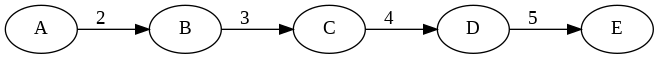
\includegraphics[width=0.9\columnwidth]{fig/naive_graph.png}
    
    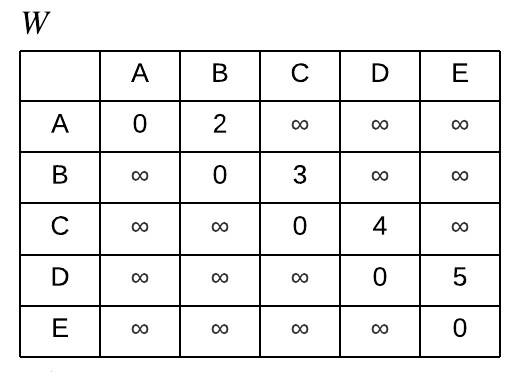
\includegraphics[width=0.4\columnwidth]{fig/DP_shortest_paths.png}
        \caption{The simple graph and its adjacency matrix representation (changing it to lower letter)}
    \label{fig:naive_graph}
\end{figure}

\paragraph{Overlapping Subproblems and Optimal Substructures} For all-pair shortest paths, we have $|V|^2$ optimal subproblems, each subproblem $D{(i,j)}$ is defined as the shortest-path between $v_i$ and $v_j$. Optimal Substructures states ``\textit{the optimal solution to a problem has the optimal solutions to subproblems in it}.'' 
%Use the bottom-up approach, the core of dynamic programming is the smaller subproblems constituent larger subproblems, and the subproblems overlap in the sense that they can be used multiple times to constituent multiple larger subproblems.
All of this boils down to how to define the ``subproblem'' and how a larger subproblem is divided into smaller subproblems (the recurrence relation).

With our naive directed graph, the shortest path between $a$ and $d$ come from the shortest path between $a$ to an intermediate node $x$ or the shortest path between $a$ and $d$ found so far. First, we define the subproblem as the shortest path between $a$ and $d$ with maximum path length(MPL) $m$. With this definition, we show two possible ways of dividing the subproblem:
\begin{enumerate}
    \item  We divide a subproblem with MPL $m$ into a subproblem with MPL $m-1$ and an edge. Therefore, the shortest path at this maximum length $m$ is either the shortest path found so far or equals to the shortest path between $a$ and $x$ plus the weight of edge $(x,d)$, our recurrence relation is:
    \begin{align}
    D^{m}{(a,d)} = \min_x(D^{m-1}{(a,d)}, D^{m-1}{(a,x)}+W{(x,d)})
    \label{eq:dp_1}
    \end{align}
    As we can see, each update for an item in distance matrix $D$ takes $O(|V|)$ time as it has to check all possible intermediate nodes. Furthermore, it takes $|V|-1$ passes to update $D^{0}$ all the way to $D^{|V|-1}$. Therefore, this approach has a time complexity of $O(|V|^4)$. We demonstrate the update process in  Fig.~\ref{fig:dp_1} for our naive example.
    \begin{figure}[!ht]
    \centering
    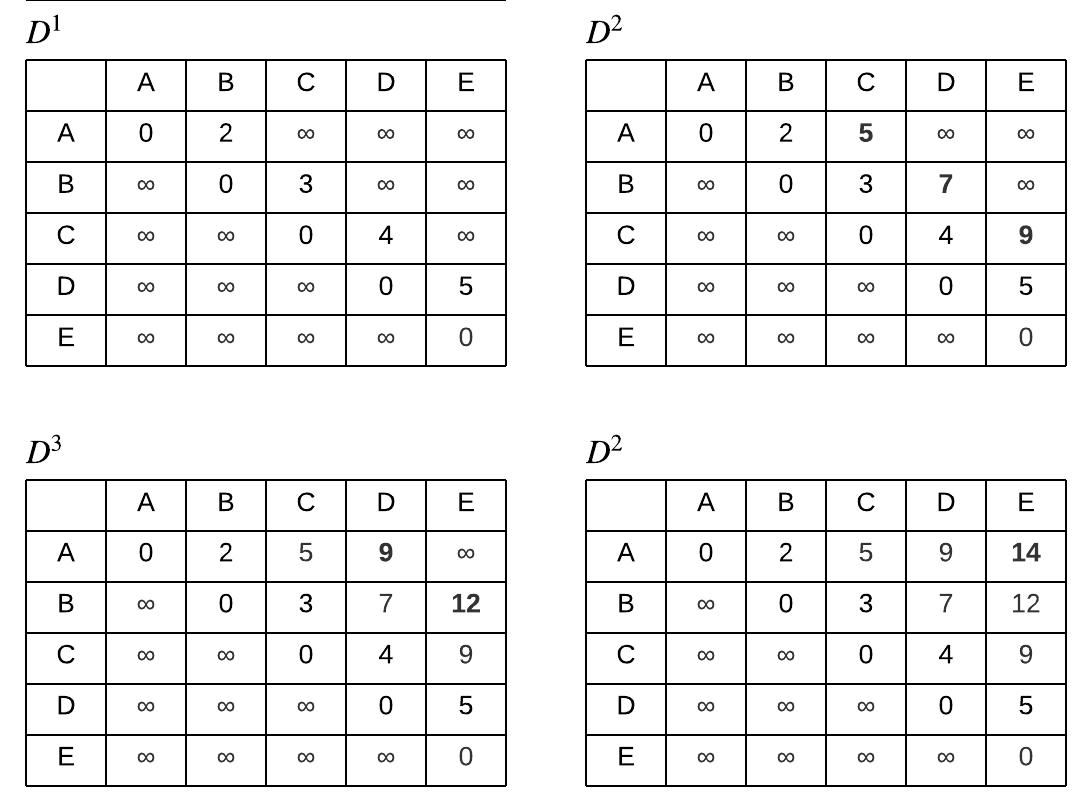
\includegraphics[width=0.8\columnwidth]{fig/DP_shortest_paths (1).png}
        \caption{DP process using Eq. ~\ref{eq:dp_1} for Fig.~\ref{fig:naive_graph}}
    \label{fig:dp_1}
\end{figure}
    \begin{figure}[!ht]
    \centering
    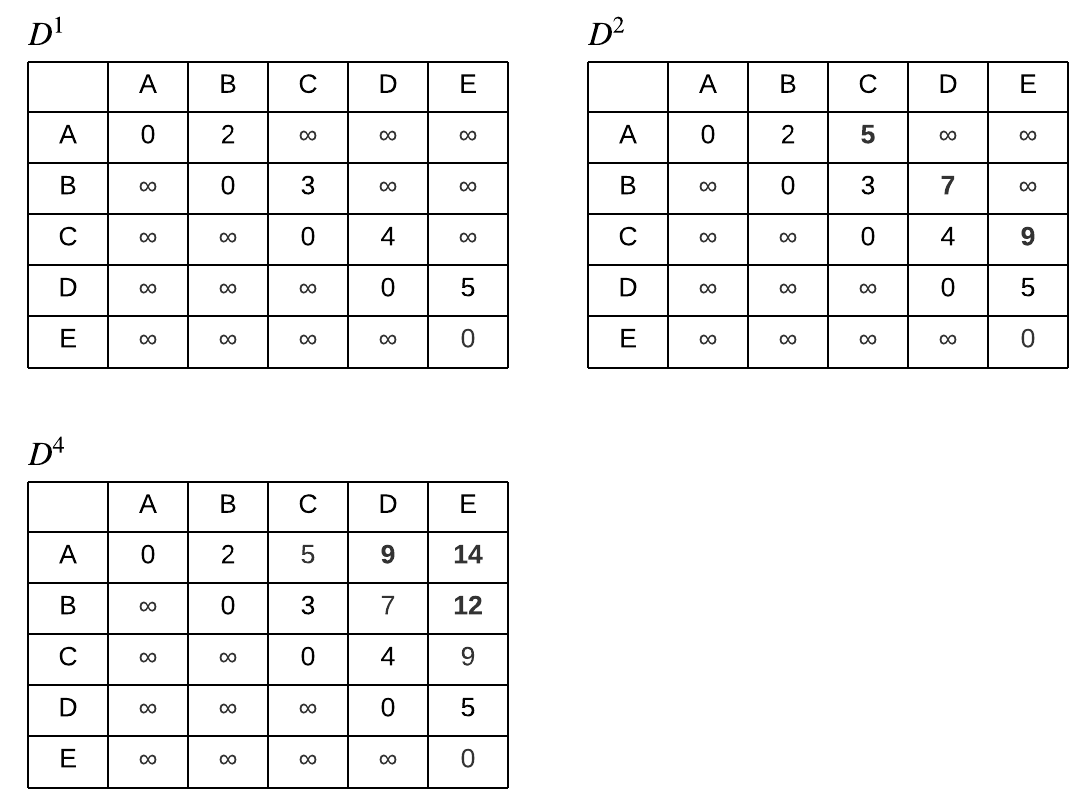
\includegraphics[width=0.9\columnwidth]{fig/DP_shortest_paths (2).png}
        \caption{DP process using Eq. ~\ref{eq:dp_2} for Fig.~\ref{fig:naive_graph}}
    \label{fig:dp_2}
\end{figure}
    \item We divide a subproblem with MPL $m$ into two equal sized subproblem, each with MPL $m/2$. Therefore, the shortest path at this maximum length $m$ is either the shortest path found so far or equals to the shortest path between $a$ and $x$ of length $m/2$ plus the shortest path between $x$ and $d$ of length $m/2$. With recurrence relation:
    \begin{align}
    D^{m}{(a, d)} = \min_x(D^{m/2}{(a,d)}, D^{m/2}{(a,x)}+D^{m/2}{(x,d)})
    \label{eq:dp_2}
    \end{align}
    Similarly, each update takes $|V|$ time. Differently, it only takes $\log |V|$ updates to get the final optimal subproblems. Thus, this approach gives a better time complexity,  $O(|V|^3\log|V|)$.  The process is demonstrated in Fig.~\ref{fig:dp_2}.
\end{enumerate}

Alternatively, we define the subproblem as the shortest path between $a$ and $d$ with $x$ as an intermediate node along the path, the number of intermediate node is $|V|$. Here, we use $k$ to index the intermediate node, and $i$, $j$ to index the start and end node. Then a subproblem $D^{k}{(i,j)}$ can be either the shortest path between $i$ and $j$ with intermediate nodes ${0, 1, ..., k-1}$ or the shortest path between $i$ and $k$ with all previous intermediate nodes plus the shortest path between $k$ and $j$ with all previous intermediate nodes. The recurrence relation is:%between $A$ and $D$ with $|V|$ possible intermediate nodes.
    \begin{align}
    D^{k}{(i,j)} = \min(D^{\{0, ..., k-1\}}{(i,j)}, D^{\{0,..., k-1\}}{(i,k)}+D^{\{0,..., k-1\}}{(k,j)})
    \label{eq:dp_3}
    \end{align}
As we see, each recurrence update only takes constant time. At the end, after we consider all possible intermediate nodes, we reach out to the optimal solution. This approach results in the best time complexity, $O(|V|^3)$ so far. We demonstrate the update process in Fig.~\ref{fig:dp_3}.  At pass $C$, using $C$ as intermediate node, we end up only use $C$-th row and $C$-th column to update our matrix.
\begin{figure}[!ht]
    \centering
    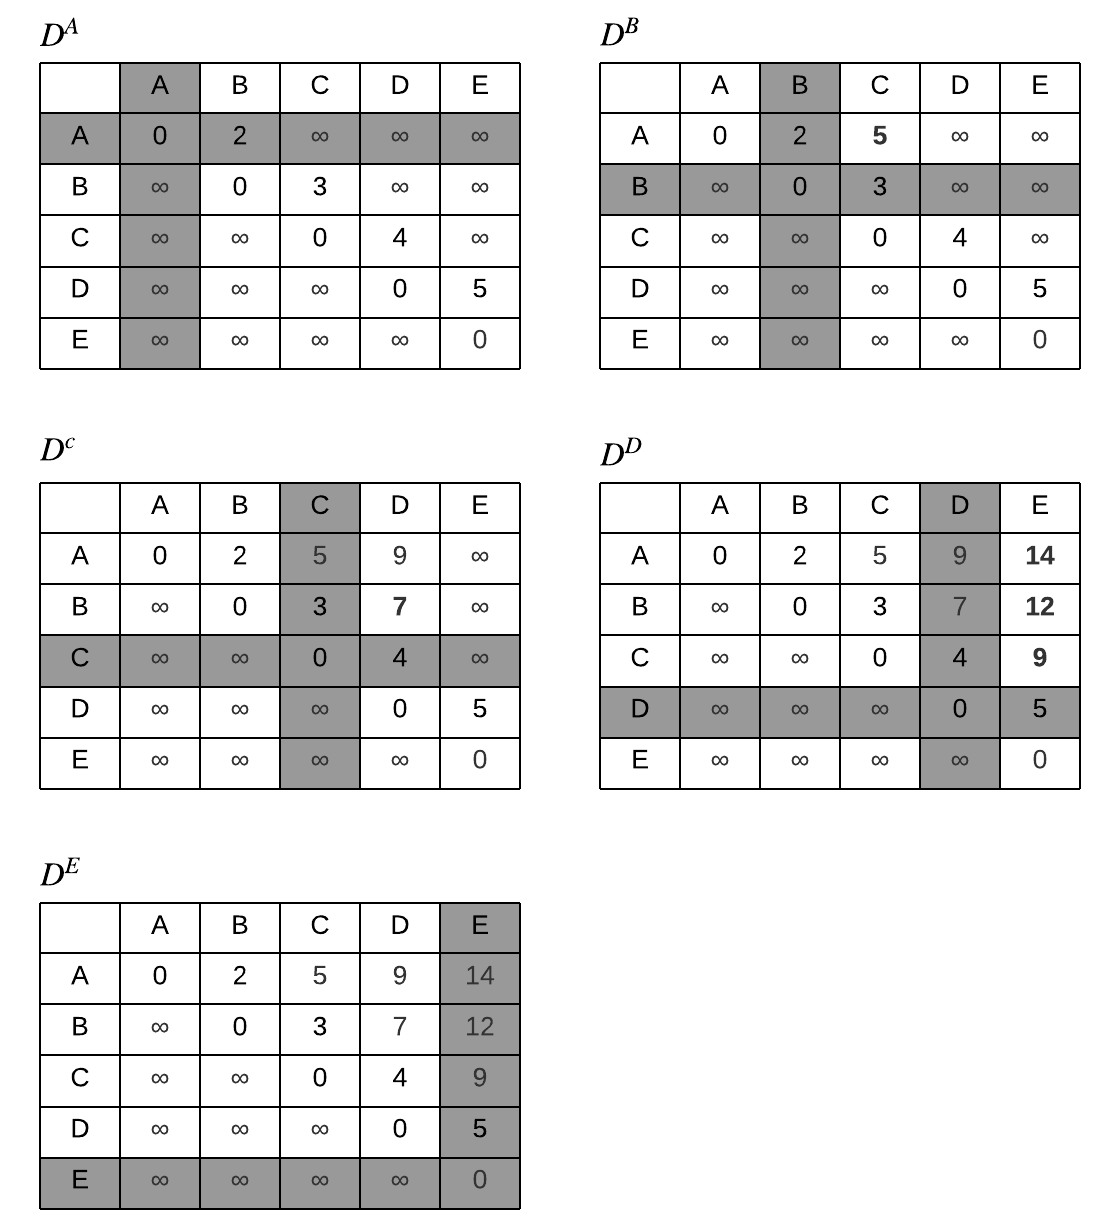
\includegraphics[width=0.8\columnwidth]{fig/chapter_advanced_graph/DP_shortest_paths (3).png}
        \caption{DP process using Eq. ~\ref{eq:dp_3} for Fig.~\ref{fig:naive_graph}}
    \label{fig:dp_3}
\end{figure}

As we shall see later, the first way is similar to Bellman-Ford, the second is a repeated squaring version of Bellman-Ford, and the third is Floyd-warshall algorithm.

\paragraph{Greedy algorithms} For $|V|^2$ subproblems, solving each subproblem takes at least $|V|$ using Floyd-warshall algorithm. Greedy approach would think of ways to decide the optional solution to each subproblem in one try, making it $|V|^2$ or $|V|+|E|$. We will see Dijkstra algorithm which is only applicable on all positive weighted $W$. 



% \paragraph{Overlapping Subproblems} For any path $(v_0,..., v_{k})$ with $k$ edges, it can be split into subpaths. There exists many ways to do it: we can split it into 2 to $k$ subpaths, and each one's path length varies. If we set the number of subpaths to 2:
% \begin{itemize}
%     \item One subpath be $(v_0, ..., v_{k-1})$ will be of length $k-1$ and the other  subpath is left with length $1$.
%     \item Assume $k$ is an even number, we decompose the path into half and half, each of length $k/2$.
% \end{itemize}

% In the single-source shortest-path problem, there lies $|V|-1$ number of subproblems, denoted as:
% \begin{align}
% \{ s \xrightarrow[]{\text{p}} v \text{ } | \text{ } v \in V, v\neq s \}
% \end{align}
% Each subproblem  $ s \xrightarrow[]{\text{p}} v$ represents all paths between $s$ and $v$ and along each one's path weight. Using the first type of decomposition shown above, this subproblem can be resolved through subproblems:
% \begin{align}
%     s \xrightarrow[]{\text{p}} v \text{ } =  s \xrightarrow[]{\text{p}} u, (u, v) \text{ },  \text{ } u \in V,
%     \label{eq_sp_subp}
% \end{align}
% where $(u, v)$ is edge incident to $v$ (explain incident in graph). For example, in Fig.~\ref{fig:sp_udg}, vertex $z$ has two incident edges $(y, z)$ and $(t, z)$, the paths between $s$ and $z$ can be obtained from subpaths:  $s \xrightarrow[]{\text{p}} y, (y, z)$ and $s \xrightarrow[]{\text{p}} t, (t, z)$. From the search tree, we can also clearly see that conclusion. 

% Also, in our problem, some subproblems are used repeatedly to reconstruct a larger subproblem. For example, $s \xrightarrow[]{\text{p}} y$ is used to get $s \xrightarrow[]{\text{p}} x$, $s \xrightarrow[]{\text{p}} z$. These are the overlapping subproblems property applied in shortest-path context. 
% \paragraph{Optimal Substructures}
% Optimal Substructures states ``\textit{the optimal solution to a problem has the optimal solutions to subproblems in it}.'' Using our example, as shown in the shortest paths in Fig.~\ref{fig:sp_udg}, the optimal solution between $s$ and $z$ has other optimal solutions: $\sigma(s, t), \sigma(s, x), \sigma(s, y)$.  But, specifically with the decomposition shown in Eq.~\ref{eq_sp_subp}, our optimal substructure is:
% \begin{align}
%     \sigma(s, v) = \min_u (\sigma(s, u) + w(u, v))
%     \label{eq_optimal_substructure}
% \end{align}




% \paragraph{Greedy algorithms} For $|V|^2$ subproblems, solving each subproblem takes at least $|V|$ using bell-man ford. Greedy approach would think ways to decide the optional solution to each subproblem in one try, making it $|V|^2$ or $|V|+|E|$. We will see Dijkstra algorithm which is only applicable on all positive weighted $W$. 

In the following section, we start with going through algorithms solving single-source shortest path problem  before we put up more details to the all-pair shortest path algorithms introduced above.

\subsection{The Bellman-Ford Algorithm}
\label{subsec_bellman_ford}
Bellman-ford algorithm addresses single-source shortest path problem using a single-source version of DP approach one.
\paragraph{Dynamic Programming Representation}
Given a single source node $s$ in graph $G$, we define $D$ and $\Pi$ as just a one-dimensional vector instead of a matrix in all-pair shortest paths. $D^{m}_i$ represents the shortest path between $s$ and $i$ with maximum path length $m$. When $m=0$, there is a shortest path from $s$ to $v$ with no edge iff $s=v$.
\begin{align}
     D^{0}_{i} = \left\{ 
    \begin{array}{ll}
   0 & \mbox{if   } s=i  \\
    \infty &\mbox{otherwise}
    \end{array}
    \right.
\label{eq_shortest_path_start}
\end{align}
Similarly, $\Pi^0$ is initialized as \texttt{None}. Our simplified recurrence relation is: 
\begin{align}
    D^{m}_{i} &= \min (D^{m-1}_{i}, \min_{k, k\in [0, n-1]}(D^{m-1}_{k}+W{(k, i)}))
\end{align}
% where $u$ enumerates all possible intermediate nodes. When $u=v$, $w_{(v,v)}=0$, the first item equals to the second in the first parenthesis. Further, omit the starting node $s$, the recurrence relation can be simplified as:
which can be further simplified to:
\begin{align}
    D^{m}_{i} &= \min_{k, k\in [0, n-1]}(D^{m-1}_{k}+W{(k, i)})
    \label{eq_sp_dp}
\end{align}

 In Eq.~\ref{eq_sp_dp}, once an intermediate node is found to have smaller tentative path weight than the current's value,  we set $\Pi(i)=k$.
\paragraph{Implementation}  In function \texttt{bellman\_ford\_dp}, $W$ is an $n\times n$ adjacency matrix. In the first \texttt{for} loop, we run recurrence relation in Eq.~\ref{eq_sp_dp} for $|V|-1$ passes, giving the fact that other than the negative-weight cycle, there will be at most $|V|-1$ edges for all paths within the graph.
\begin{lstlisting}[language=Python]
def bellman_ford_dp(s, W):
  n = len(W)
  # D, pi
  D = [float('inf') if i!=s else 0 for i in range(n)] # * n
  P = [None] * n
  for m in range(n-1): 
    newD = D[:]
    for i in range(n): # endpoint
      for k in range(n): # intermediate node
        if D[k] + W[k][i] < newD[i]:
          P[i] = k
          newD[i] = D[k] + W[k][i]

    D = newD
    print(f'D{m+1}: {D}')
  return D, P
\end{lstlisting}
Now, to retrieve the path from source $s$ to other vertices, we implement a recursive function named \texttt{get\_path} that starts from the target $u$ and backtraces to the source $s$ through  $\Pi$. The code is as:
\begin{lstlisting}[language=Python]
def get_path(P, s, u, path):
  path.append(u)
  if u == s:
    print('Reached to the source vertex, stop!')
    return path[::-1]
  elif u is None:
    print(f"No path found between {s} and {u}.")
    return [] 
  else:  
    return get_path(P, s, P[u], path)
\end{lstlisting}
For the graph in Fig.~\ref{fig:sp_udg}, the updating on $D$ using $s$ as source is visualized in Fig.~\ref{fig:bellman_ford_1}. 
\begin{figure}[!ht]
    \centering
    % \begin{subfigure}{.32\textwidth}
    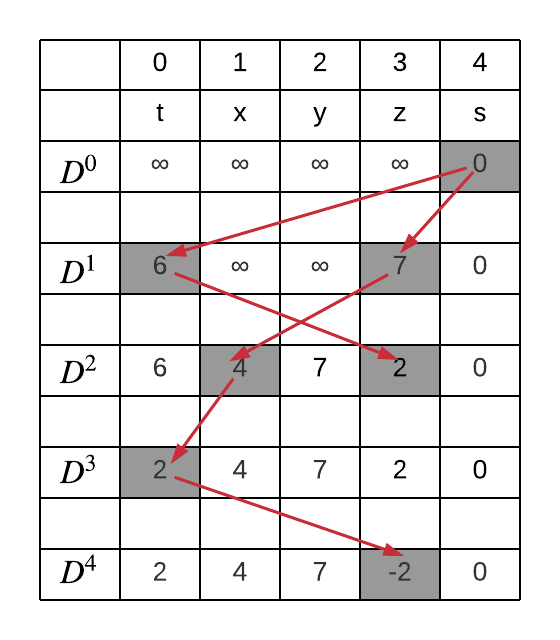
\includegraphics[width=0.4\columnwidth]{fig/bellman-ford-D (2).png}
    % \caption{Initialization}
    % \end{subfigure}
    % \begin{subfigure}{.32\textwidth}
    % 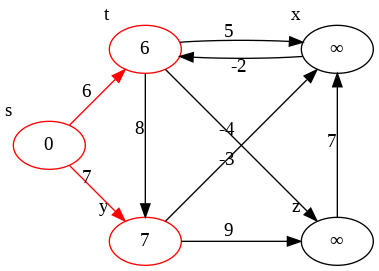
\includegraphics[width=0.99\columnwidth]{fig/bellman_ford_1.png}
    % \caption{After $1^{st}$ Pass}
    % \end{subfigure}
    % \begin{subfigure}{.32\textwidth}
    % 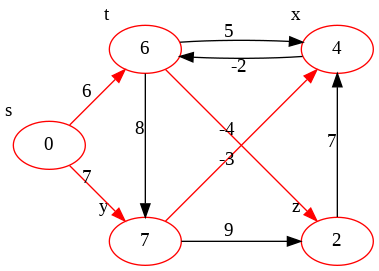
\includegraphics[width=0.99\columnwidth]{fig/bellman_ford_2.png}
    % \caption{After $2^{nd}$ Pass}
    % \end{subfigure}
    
    % \begin{subfigure}{.32\textwidth}
    % 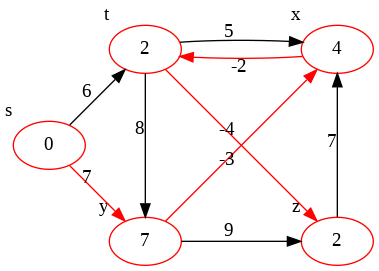
\includegraphics[width=0.99\columnwidth]{fig/bellman_ford_3.png}
    % \caption{After $3^{rd}$ Pass}
    % \end{subfigure}
    % \begin{subfigure}{.32\textwidth}
    % 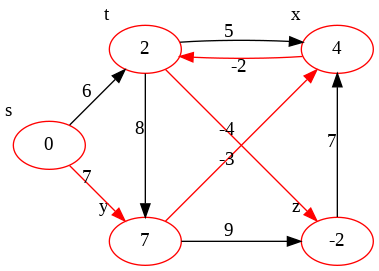
\includegraphics[width=0.99\columnwidth]{fig/bellman_ford_4.png}
    % \caption{After $4^{th}$ Pass}
    % \end{subfigure}
    \caption{The update on $D$ for Fig.~\ref{fig:sp_udg}. The gray filled spot marks the nodes that updated its estimate value, with its precessor indicated by incoming red arrow.}
    \label{fig:bellman_ford_1}
\end{figure}
Connecting all red arrows along with the shaded gray nodes, we have a tree structure, each update on $D$, we expand the tree by one more level, updating the best estimate reaching to target node with one more possible edge. We visualize this tree structure in Fig.~\ref{fig:bellman_ford_2}. We explain the tree like this: if we are at most one edge away from $s$, we get $t$ as small as $6$, if we are three edges away, $t$ is able to gain a smaller value through its predecessor $x$ which is at most 2 edges away. After the last round of update, when the tree reaches to height $|V|-1$, the predecessor vector $\Pi$ will gives out the shortest-path tree: each edge in the shortest path tree can be obtained by connecting each predecessor with vertices in the graph. The shortest-path tree is marked in Fig.~\ref{fig:bellman_ford_2} in red color.
\begin{figure}[!ht]
    \centering
    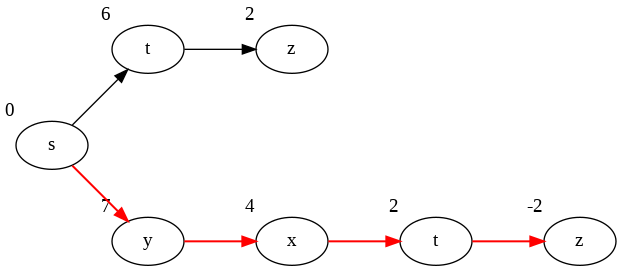
\includegraphics[width=0.7\columnwidth]{fig/shortest_path_dp_1.png}
    \caption{The tree structure indicates the updates on $D$, and the shortest path tree marked by red arrows. }
    \label{fig:bellman_ford_2}
\end{figure}
\paragraph{Formal Bellman-Ford Algorithm}
In the above implementation, at each round, we made a copy of $D$, which is named \texttt{newD}. However, we can actually reuse the original $D$ and update directly on it. The difference is: we would update \texttt{D[i]} at step $m$ with other \texttt{D[k]} at step $m$ instead of at step $m-1$, making some nodes' optimal estimate even more optimal. In the previous implementation, we can guarantee that after iteration $i$, for all $i \in [0, n-1]$, $D_i$ is at most the weight of every path from $s$ to $i$ using at most $m$ edges. In the new version, we end up reaching to the optimal value even earlier, but still it takes $n-1$ passes to guarantee. 
% \begin{align}
%     d_v \leq \min(w(p)): |p| \leq i-1,
% \end{align}%However, this doesnt matter since once it reaches to $|V|-1$ updates, the result will never change again.
% Updating in the same $D$ would only decrease $d_v$, so that the above inequation still remains true.

Second, the inner two \texttt{for} loops are equivalently enumerating edges: for each possible edge $(k, i)$, we update the best estimate for node $i$. With such two points modified, we get our official the Bellman-Ford algorithm, which states:
\begin{enumerate}
    \item Initialize $D$ and $\Pi$ as $D^{0}$ and $\Pi^0$.
    \item Run a relaxation process for $|v|-1$ passes. Within  each pass, go through each edge $(u, v) \in E$, with Eq.~\ref{eq_sp_dp}, if using $u$ as an intermediate node, the tentative shortest path has smaller value, update $D$ and $\Pi$. 
\end{enumerate}
\begin{bclogo}[couleur = blue!30, arrondi=0.1,logo=\bccrayon,ombre=true]{Implement Bellman-Ford by checking edges from adjacency list as defined in \texttt{g} for Fig.~\ref{fig:sp_udg}. We should notice that different ordering of vertices /edges to be relaxed leads to different intermediate results in $D$, though the final result is the same.} 
\end{bclogo}

\paragraph{Implementation} We give out an exemplary implementation
\begin{lstlisting}[language=Python]
def bellman_ford(g: dict, s: str):
  n = len(g)
  # Assign an enumerial index for each key
  V = g.keys()
  # Key to index
  ver2idx = dict(zip(V, [i for i in range(n)]))
  # Index to key
  idx2ver = dict(zip([i for i in range(n)], V))
  # Initialization the dp matrix with d estimate and predecessor
  si = ver2idx[s]
  D = [float('inf') if i!=si else 0 for i in range(n)] # * n
  P = [None] * n
  
  # n-1 passes
  for i in range(n-1): 
    # relax all edges
    for u in V:
      ui = ver2idx[u]
      for v, w in g[u]:
        vi = ver2idx[v]
        # Update dp's minimum path value and predecessor
        if D[vi] > D[ui] + w:
          D[vi] = D[ui] + w
          P[vi] = ui
    print(f'D{i+1}: {D}')  
  return D, P, ver2idx, idx2ver
\end{lstlisting}
During each pass, we relax on the estimation $D$ with the following ordering:
\begin{lstlisting}[numbers=none]
    's':[('t', 6), ('y', 7)],   
    't':[('x', 5), ('y', 8), ('z', -4)],
    'x':[('t',-2)],
    'y':[('x',-3), ('z',9)],
    'z':[('x',7)],
\end{lstlisting}
Printing out on the updates of $D$, we can see that it converges to the optimal value faster than the previous strict Dynamic programming version. 

\paragraph{Time Complexity} The first dynamic programming solution takes $O(|V|^3)$, and the formal Bellman-Ford takes $O(|V||E|)$. The later would be more efficient than the first if our graph is dense.
% When the ordering of edges to be relaxed e each pass is
% \begin{lstlisting}[numbers=none]
% g = {
%     't':[('x', 5), ('y', 8), ('z', -4)],
%     'x':[('t',-2)],
%     'y':[('x',-3), ('z',9)],
%     'z':[('x',7)],
%     's':[('t', 6), ('y', 7)],   
% },
% \end{lstlisting}
% The process of Bellman-Ford algorithm is visualized in Fig.~\ref{fig:bellman_ford_1} on a directed graph shown in Fig.~\ref{fig:sp_udg} that contains no negative-weight cycle. 

\paragraph{Detect Negative-weight Cycle} 
% \begin{figure}
%     \centering
%     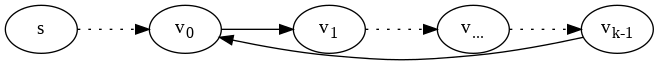
\includegraphics[width=0.95\columnwidth]{fig/path_cycle.png}
%     \caption{A path that has at least one cycle.}
%     \label{fig:path_cycle}
% \end{figure}
If the graph contains no negative-weight cycle, after $|V|-1$ passes of relaxation, $D$ will reach to the minimum path value. Thus, if we run additional pass of relaxation, no vertex would be updated further. However, if there exists at least one negative-weight cycle, the $|V|^{th}$ update will have at least one vertex in $D$ with decreased value. 
%%%%%%%%Proof%%%%%%%%%%
% Assume on a graph there is one negative-weight cycle that is reachable from source $s$; let this cycle be $c=(v_0, v_1, ..., v_{k}), v_0=v_{k}$ and $\sum_{i=1}^{k} w(v_{i-1}, v_i) <0$. Assume at the $|V|^{th}$ pass, no additional updated is detected, making $v_{i}.d \leq v_{i-1}.d +  w(v_{i-1}, v_i), i\in [1,k]$. Summing the inequalities, we get:
% \begin{equation}
%     \sum_{i=1}^{k} d_{v_{i}} \leq \sum_{i=1}^{k} d_{v_{i-1}} + \sum_{i=1}^{k}w(v_{i-1}, v_i)
% \end{equation}
% Since $v_0=v_k$, we cancel the summation of $v.d$ on each side, and get
% \begin{equation}
%     0 \leq \sum_{i=1}^{k}w(v_{i-1}, v_i)
% \end{equation}
% which contradicts with the fact that it is a negative-weight cycle. Therefore, there will be at least one vertex on the cycle that will keep decreasing its value on the $|V|^{th}$ pass. 


\subsubsection{Special Cases and Further Optimization}
From the perspective of optimization, there are at least two approaches we can try to further boost the time efficiency, such as 
\begin{enumerate}
   \item special linear ordering of vertices to relax its leaving edges that leads us to its shortest-paths in just one pass of the Bellman-Ford algorithm,
    \item and some greedy approach that takes only one pass of relaxation which can be similar to breath-first graph search or the Prim's algorithm.
\end{enumerate}
In Fig.~\ref{fig:bellman_ford_1}, suppose we are relaxing leaving edges of vertices in linear order $[s, t, y, z, x]$, the process will be as follows:
\begin{lstlisting}[numbers=none]
vertex         edges      relaxed vertices
s           (s,t),(s,y)   {t:6, y:7}
t   (t,x),(t,y),(t,z)     {x:11, z:2, t:6, y:7}
y         (y,x), (y,z)    {x:4, z:2, t:6, y:7}
z             (z,x)       {x:4, z:2, t:6, y:7}
x             (x,t)       {t:2, x:4, z:2, y:7}
\end{lstlisting}
\begin{figure}[!ht]
    \centering
    \begin{subfigure}{.45\textwidth}
    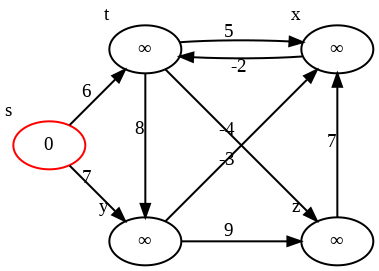
\includegraphics[width=0.99\columnwidth]{fig/bellman_ford_0_tp.png}
    \caption{Initialization}
    \end{subfigure}
    \begin{subfigure}{.45\textwidth}
    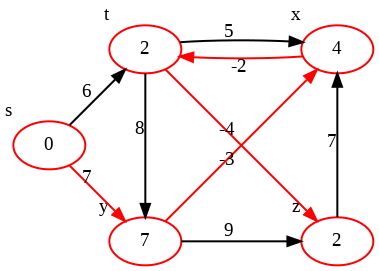
\includegraphics[width=0.99\columnwidth]{fig/bellman_ford_1_tp.png}
    \caption{After $1^{st}$ Pass}
    \end{subfigure}
    \caption{The execution of Bellman-Ford's Algorithm with ordering $[s, t, y, z, x]$.}
    \label{fig:bellman_ford_3}
\end{figure}
The process is also visualized in Fig.~\ref{fig:bellman_ford_3}.
We see that only vertex $z$ did not find its shortest-path weight. Why? From $s$ to $z$, there are paths: $(s, t, z), (s, t, z), (s, t, y, z), (s, y, x, t, z)$. If we want to make sure after one pass of updates, vertex $z$ reaches to its minimum shortest-path weight, we have to make sure its predecessors all reach to its minimum-path weight too which are vertex $y$ and $t$. Same rule applies to its predecessors. In this graph, the ordering 
\begin{lstlisting}[numbers=none]
vertex  predecessor
s       None
t      s, x
y      s, t
x     t, y, z
z    y, t
\end{lstlisting}
From the listing, we see that the pair $t$ and $x$ conflicts each other: $t$ needs $x$ as predecessor and $x$ needs $t$ as predecessor. Tracking down this clue, we will find out that it is due to the fact that $t$ and $x$ coexist in a cycle. 
\paragraph{Order Vertices with Topological Sort} 
\begin{figure}[!ht]
    \centering
    \begin{subfigure}{.45\textwidth}
    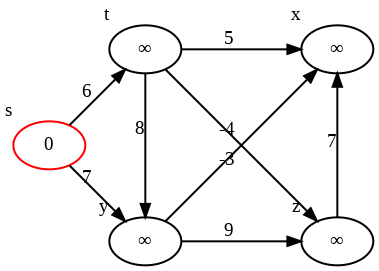
\includegraphics[width=0.99\columnwidth]{fig/bellman_ford_0_dag.png}
    \caption{Initialization}
    \end{subfigure}
    \begin{subfigure}{.45\textwidth}
    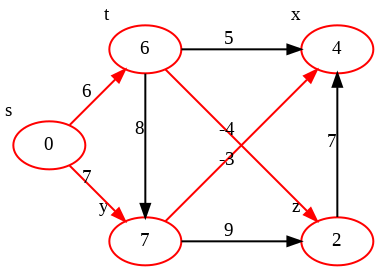
\includegraphics[width=0.99\columnwidth]{fig/bellman_ford_1_dag.png}
    \caption{After $1^{st}$ Pass}
    \end{subfigure}
    \caption{The execution of Bellman-Ford's Algorithm on DAG using topologically sorted vertices. The red color marks the shortest-paths tree.}
    \label{fig:bellman_ford_2}
\end{figure}
Taking away edge $(x, t)$, we are able to obtain a topological ordering of the vertices, which is $[s, t, y, z, x]$. Relaxing vertices by this order of its leaving edges will guarantee to reach to the global-wise shortest-path weight that would otherwise be reached in $|V|-1$ passes in Bellman-Ford algorithm using arbitrary ordering of vertices. The shortest-paths tree is shown in Fig.~\ref{fig:bellman_ford_2}.

So far, we discovered a $O(|V|+|E|)$ linear algorithm for single-source shortest-path problem when the given graph being directed, weighted, and acyclic. The algorithm consists of two steps: topological sorting of vertices in $G$ and one pass of Bellman-Ford algorithm using the reordered vertices instead of arbitrary ordering. Calling the \texttt{topo\_sort} function from Section.~\ref{sec_topological_sort}, we have our Python code:
\begin{lstlisting}[language=Python]
def bellman_ford_dag(g, s):
  s = s
  n = len(g)
  # Key to index
  ver2idx = dict(zip(g.keys(), [i for i in range(n)]))
  # Index to key
  idx2ver = dict(zip([i for i in range(n)], g.keys()))
  # Convert g to index
  ng = [[] for _ in range(n)]
  for u in g.keys():
    for v, _ in g[u]:
      ui = ver2idx[u]
      vi = ver2idx[v]
      ng[ui].append(vi)
  V = topo_sort(ng)
  # Initialization the dp matrix with d estimate and predecessor
  si = ver2idx[s]
  dp = [(float('inf'), None) for i in range(n)]
  dp[si] = (0, None)

  # relax all edges
  for ui in V:
    u = idx2ver[ui]
    for v, w in g[u]:
      vi = ver2idx[v]
      # Update dp's minimum path value and predecessor
      if dp[vi][0] > dp[ui][0] + w:
        dp[vi] = (dp[ui][0] + w, ui)
  return dp
\end{lstlisting}
\subsection{Dijkstra's Algorithm}
\label{subsec_dijkstra}
\paragraph{From Prim's to Dijkstra's} In Breath-first Search, it hosts a FIFO queue, and whenever the vertex finishes exploring and turns into BLACK color, it is guaranteed to have the shortest-path length from the source. Similarly, in Prim's algorithm, it maintains a priority queue of cross edges between the spanning tree set $S$ and the remaining set $V-S$, whenever a vertex is added into $S$, it is a part of the MST. 

In the shortest-path problem, using the same initialization in Bellman-Ford algorithm, that source vertex has $0$ estimate to the source and all other vertices take $\infty$. Following the process of Prim's algorithm, we set a set $S$ to save vertices that has found its shortest-path weight and predecessor, which is empty initially. Then, the algorithm starts the from the ``lightest'' vertex in $V-S$ to add to the set $S$, which is source vertex $s$ at first, and it relax on the shortest-path estimate of vertices that are the endpoints of edges leaving the lightest vertex. This process is repeated in a loop until $V-S$ is empty. This devised approach indeed follows the principle of greedy algorithm just as Prim's algorithm does, this algorithm is called \textit{Dijkstra's}.

\paragraph{How is it greedy?} Dijkstra's is the ``greedy'' version of Bellman-ford Algorithm. At each step, dynamic programming uses Eq.~\ref{eq_sp_dp} to update $D^{m}_i$ by trying all possible edges that extend the paths between $s$ and $i$ one at a time. Bellman-ford can only guarantee to achieve the optimal solution at the very end of running all passes.  However, in Dijkstra algorithm, it reaches to the optimal solution in only one step--whenever a vertex is added into $S$, it adds a vertex in the shortest-path tree with only ``local'' information. 
%-optimal substructures indicates that we can extend from vertices that have reached to its minimum path estimate to its adjacent vertices through outgoing edges. 

\paragraph{Correctness Condition: Non-negative Weight}  But, how to make sure that whenever the vertex was added into set $S$, it reaches to its shortest-path weight? Specifically, how to ensure our locally optimal decision is global optimal?
%, that when a vertex $u$ is added into $S$, its estimated shortest-path weight is $\sigma(s, u)$. 
This also means after this step, no matter how many additional paths with larger path length can reach to $i$, they shall never have less distance. This requires all of graph edges to be non-negative. 
\begin{figure}[!ht]
    \centering
    \begin{subfigure}{.32\textwidth}
    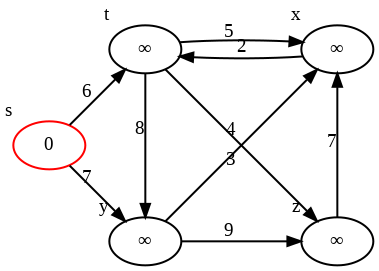
\includegraphics[width=0.99\columnwidth]{fig/dijkstra_0.png}
    \caption{$s$ enters Queue}
    \end{subfigure}
    \begin{subfigure}{.32\textwidth}
    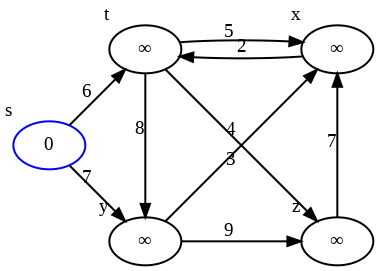
\includegraphics[width=0.99\columnwidth]{fig/dijkstra_0.5.png}
    \caption{$s$ enters $S$}
    \end{subfigure}
    \begin{subfigure}{.32\textwidth}
    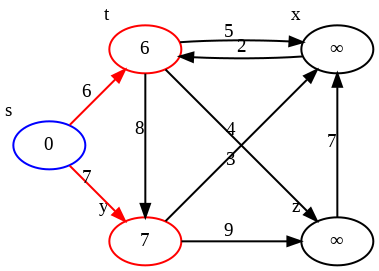
\includegraphics[width=0.99\columnwidth]{fig/dijkstra_1.png}
    \caption{$t$ and $y$ enter Queue}
    \end{subfigure}
    

    \begin{subfigure}{.32\textwidth}
    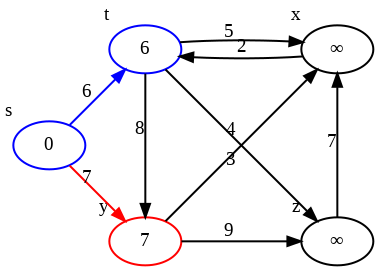
\includegraphics[width=0.99\columnwidth]{fig/dijkstra_1.5.png}
    \caption{$t$ enters $S$}
    \end{subfigure}
    \begin{subfigure}{.32\textwidth}
    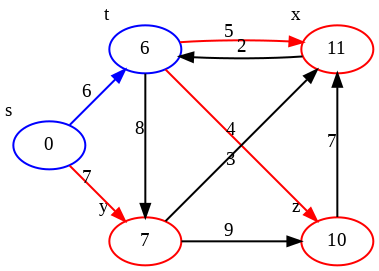
\includegraphics[width=0.99\columnwidth]{fig/dijkstra_2.png}
    \caption{$z$ and $x$ enter Queue}
    \end{subfigure}
    \begin{subfigure}{.32\textwidth}
    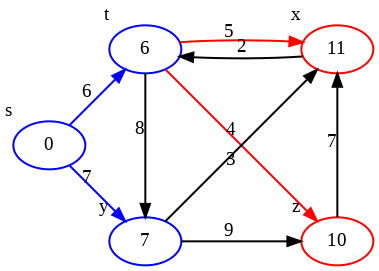
\includegraphics[width=0.99\columnwidth]{fig/dijkstra_2.5.png}
    \caption{$y$ enters $S$}
    \end{subfigure}
    \begin{subfigure}{.32\textwidth}
    
    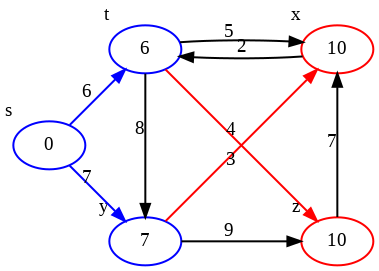
\includegraphics[width=0.99\columnwidth]{fig/dijkstra_3.png}
    \caption{$x$ is modified in Queue}
    \end{subfigure}
        \begin{subfigure}{.32\textwidth}
    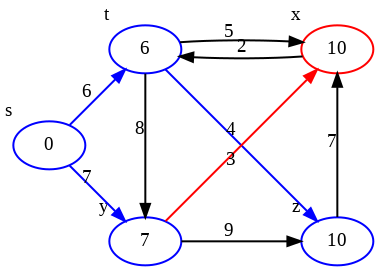
\includegraphics[width=0.99\columnwidth]{fig/dijkstra_3.5.png}
    \caption{$z$ enters $S$}
    \end{subfigure}
        \begin{subfigure}{.32\textwidth}
    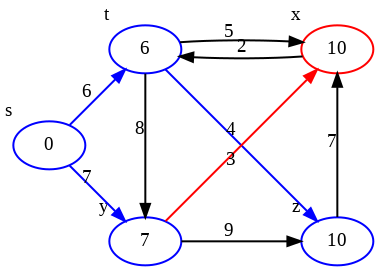
\includegraphics[width=0.99\columnwidth]{fig/dijkstra_4.png}
    \caption{Queue is not modified}
    \end{subfigure}
    
        \begin{subfigure}{.32\textwidth}
    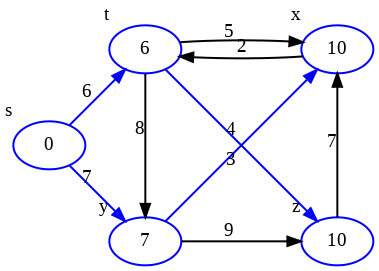
\includegraphics[width=0.99\columnwidth]{fig/dijkstra_4.5.png}
    \caption{$x$ enters $S$}
    \end{subfigure}
    \caption{The execution of Dijkstra's Algorithm on non-negative weighted graph. Red circled vertices represent the priority queue, and blue circled vertices represent the set $S$. Eventually, the blue colored edges represent the shortest-paths tree.}
    \label{fig:dijikstra}
\end{figure}
\paragraph{Implementation}

The implementation relies on the \texttt{PriorityQueue()} customized data structure once again, where we can modify an existing item in the queue. There are two ways to apply the priority queue:
\begin{itemize}
    \item Add all vertices into the queue all at once at the beginning. Then only \texttt{deque} and modification operations are needed. 
    \item Add vertex in the queue only when it is relaxed and has a non-$\infty$ shortest-path estimate. The process of Dijkstra algorithm on a non-negative weighted graph that takes this approach of queue is demonstrated  in Fig.~\ref{fig:dijikstra} and the code is as follows:
\end{itemize}
\begin{lstlisting}[language=Python]
def dijkstra(g, s):
  Q = PriorityQueue()
  S = []
  # task: vertex id, priority: shortest-path estimate, info: predecessor
  Q.add_task(task=s, priority=0, info=None)
  visited = set()
  while not Q.empty():
    # Use the light vertex
    u, up, ud = Q.pop_task()
    visited.add(u)
    S.append((u, ud, up))

    # Relax adjacent vertice
    for v, w in g[u]: 
      # Already found the shortest path for this id
      if v in visited: 
        continue
      
      vd, vp = Q.get_task(v)
      # First time to add the task or already in the queue, but need update 
      if not vd  or ud + w < vd:
        Q.add_task(task=v, priority=ud + w, info=u)
  return S
\end{lstlisting}


% \paragraph{Correctness of Dijkstra's Algorithm}
% To prove the correctness of a greedy algorithm is not easy matter, and often the contradiction method can be used. In this process, we need to show that for each vertex $u\in V$, we have $u.d = \sigma(s, u)$ at the time when $u$ is added to set $S$.
% \begin{figure}[!ht]
%     \centering
%     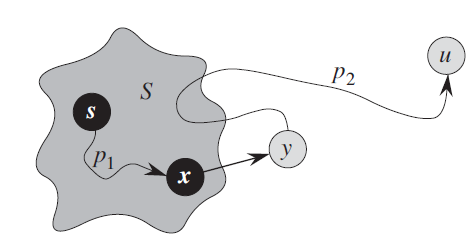
\includegraphics[width=0.5\columnwidth]{fig/dijkstra_proof.png}
%     \caption{The proof of correctness of Dijkstra's Algorithm}
%     \label{fig:dijkstra_proof}
% \end{figure}
% \begin{enumerate}
%     \item Initialization: First, $S=\emptyset$, the conclusion holds true. 
%     \item Maintenance: We wish to show that in each iteration, $u.d=\sigma(s,u)$ for the vertex added to set $S$. We use contradiction, let $u$  be the first vertex for which $u.d\neq\sigma(s,u)$. For this to work, $u$ cant be $s$ and it also needs to be a vertex that is reachable from $s$. Importantly, if $u.d\neq\sigma(s,u)$, then there shall exist another path, namely $s\rightarrow x \rightarrow y \rightarrow u$ is shorter. We set the context of one step before, that prior to adding $u$ to $S$, path $p$ connects $s$ to  a vertex is in $S$, namely $x$ in $V-S$. At this step, because of induction, $p_1 = s\rightarrow x$ is $\sigma(s,x)$.  Edge (x, y) is relaxed at that time. 
    
%     First, because $y$ appears before $u$ on the shortest-path on shortest path $s \rightarrow u$, and all edges are non-negative, we have:
%     \begin{align}
%         \sigma(s,y) &\leq \sigma(s, u), \\
%         y.d &= \sigma(s,y) \\
%         y.d &\leq u.d
%     \end{align}
    
%     Because, both vertices $u$ and $y$ were in $V-S$ when $u$ was added, we have $u.d\leq y.d$ since we chose $u$ instead. Thus we get an equality
%     $y.d = \sigma(s, y) = \sigma(s, u) = u.d$
% \end{enumerate}

% There is another version reasoned with non-decreasing property:  
% \begin{enumerate}
% \item At the first pass, we start from the source vertex, which is a shortest path itself with weight $0$. The next we do it to relax edges that out of the source vertex, and among them, we choose the shortest path. Because of the non-decreasing property, that if $v^{*}_i$ is the minimum at this step, then all other possible paths that reaches to  $v^{*}_i$ through ${S_{v_l}-v^{*}_i}$ will has longer length, there weight will only increase,  such that it will never come back to harness the current decision. 
%     \item At the second step, we follow the same rule, relax the edges out of $v^{*}_i$. Then we have a selection of paths are one and two length away.  we would be able to finalize the shortest path from $s$ to one vertex $v^{*}_i$ by comparing the minimum weights of all of the reachable vertices. 
% \end{enumerate}
% ,  Once we make the decision, we do not need to relax weights through the whole vertex set other than relaxing the weights of reachable vertices through the current smallest vertex. This is due to the optimal substructure property.

% For example, in Fig.~\ref{}, shown in (b) at the first pass, we can decide the shortest-path between $s$ and $y$. The next pass, we only relax the path weights of $t,x, z$ that is reachable through $t$. Now, we have information of the path weights for those paths that have maximum length of 2. Then vertex $z$'s shortest path will be finalized. And so on.



\paragraph{Complexity  Analysis}
Once again, the complexity of Dijkstra's relies on the specific implementation of the priority queue.  In our implementation, we used a customized \texttt{PriorityQueue()} which takes $|V|$ to initialize the queue. In this queue, we did not really remove the task from the queue but instead  marked it as ``REMOVED,'' so we can end up having maximum of $|E|$ vertices in the queue, making the cost of extracting the minimum item   be $O(\log |E|)$. For the update, the main cost comes from inserting an new vertex through \texttt{heappush-like} operation, which is $O(\log |E|)$ too. In all, we have $|V|$ times of \texttt{pops} and $|V|$ times of updates, ending up with a worst-case time complexity of $O(|V|\log |E|)$.

\begin{bclogo}[couleur = blue!30, arrondi=0.1,logo=\bccrayon,ombre=true]{Try to prove the correctness of Dijkstra's using greedy algorithms' two approaches on proving.} 
\end{bclogo}
% \subsubsection{Implementation}
% Same as of Bellman-Ford's algorithm with the initialization, an relaxation process. 

% In Dijkstra, we separate two sets of vertices. One set $S$ whose final shortest-path weights from the source $s$ have already been decided. And the other set $V-S$ waiting to be decided. Each step, we only need to relax edges reachable to the current smallest vertices, instead of relax edges reachable through all previous relaxed edges. Once we decide it is the smallest, this vertex will be removed from set $V-S$, and add into $S$. We can use a pseudo-code to represent it simply first:
% \begin{lstlisting}
% Dijkstra(G, w, s):
%     initialize-single-source(G, s)
%     S = {}
%     Q = G.V
%     while Q not empty:
%         u=extract_min(Q)
%         S = S + {u}
%         for each vertex v in G.adj[u]:
%             Relax(u, v, w)
% \end{lstlisting}
% Now, let us implement Dijkstra's algorithm with Python. 



\subsection{All-Pairs Shortest Paths}
\label{sec_all_pairs_shortest_paths}
In this section, we first summarize the solutions to singe-source shortest-path problem due to the fact that the problem of finding all-pairs shortest-path problem can be naturally decomposed into $|V|$ such single sourced subproblems. Next, we systematically build into three all-pair paths algorithms we are about to learn: 

\paragraph{Summary to Single-source Shortest-Path Algorithms} The solutions vary to the type of weighted graph $G$ that we are dealing with:
\begin{itemize}
    \item if (1) each weight $w \in R$ and (2) only non-negative cycle, we can apply the generalist dynamic programming approach--Bellman-Ford Algorithm,
    \item if each weight is non-negative, i.e., $w \in R^{+}$, we take  the greedy approach--``Dijkstra's Algorithm''
    \item and (1) if the graph is acyclic and (2) only have non-negative cycles, we can run one pass of Bellman-Ford algorithm with vertices being relaxed in topologically sorted liner ordering.
\end{itemize}
Depends on which category the given graph $G$ falls into, a naive and nature solution to all-pairs shortest-path problem can be addressed by running the corresponding algorithm $|V|$ passes--once for each vertex viewed as source in a complexity scaled by $|V|$ times. 
%To serve the general case, such extended Bellman-ford algorithm will have a running time as of $O(|V|^2|E|)$, which will goes up to $O(|V|^4)$ if $G$ is dense. 
\subsubsection{Extended Bellman-Ford's Algorithm} We leverage the first DP approach in Section ~\ref{chapter_advanced_graph_sec_algorithm_design}. Define weight matrix $W$,  shortest-path weight estimate matrix $D$, and predecessor matrix $\Pi$. We have recurrence relation:
\begin{align}
    D^{m}{(i, j)} &= \min_{k\in [0, n-1] }(D^{m-1}{(i, k)}+W{(k, j)}),
    \label{eq_recurrence_extended_bellman}
\end{align}
$\Pi^{m}{(i,j)}$ is updated by:
\begin{align}
     \Pi^{m}{(i,j)} = \left\{ 
    \begin{array}{ll}
   \mbox{None,} &\mbox{if } D^{m}{(i, j)=0}  \mbox{ or } D^{m}{(i, j)} = \infty,\\
  \operatorname*{argmin}_{k \in [0, n-1]} (D^{m-1}{(i, k)}+W{(k, j)}), &\mbox{otherwise. } 
    \end{array}
    \right.
    \label{eq_bellman_predecessor}
\end{align}
with initialization:
\begin{align}
     D^{0}{(i, j)} = \left\{ 
    \begin{array}{ll}
   0, & \mbox{if   } i=j,  \\
    \infty, &\mbox{otherwise.}
    \end{array}
    \right.
\label{eq_extend_bellman_ford}
\end{align}
\begin{align}
     \Pi^{0}{(i,j)} = None
    \label{eq_bellman_predecessor}
\end{align}

% \begin{equation}
%      W{(i, j)} = \left\{ 
%     \begin{array}{lll}
%   0 & \mbox{if   } i=j  \\
%   w_{ij} & \mbox{if $i\ne j$, and  $(i, j)\in E$ } \\
%     \infty & \mbox{if $i\ne j$, and  $(i, j)\notin E$ }
%     \end{array}
%     \right.
% \end{equation} 

% , from a vector to a matrix of size $|V| \times |V|$. Each $w_{ij}$, $d_{ij}$, $\pi_{ij}$, and $\sigma_{ij}$ is defined as follows:
% \begin{itemize}
%     \item $w_{ij}$ indicates the weight of each edge with startpoint $i$ and endpoint $j$, 
% \begin{equation}
%      w{(i, j)} = \left\{ 
%     \begin{array}{lll}
%   0 & \mbox{if   } i=j  \\
%   w_{ij} & \mbox{if $i\ne j$, and  $(i, j)\in E$ } \\
%     \infty & \mbox{if $i\ne j$, and  $(i, j)\notin E$ }
%     \end{array}
%     \right.
% \end{equation} 
% \item Compared with Eq.~\ref{eq_optimal_substructure}, single source $s$ is replaced by $i$, which can be any vertex from $V$,
% \begin{align}
%     \sigma(i, j) = \min_{u \in V} (\sigma(i, u) + w{(u, j)})
% \end{align}
% \item Similarly, compared with Eq.~\ref{eq_sp_dp}, $d$  adds additional index $i$, representing the starting vertex for the path $i\rightarrow j$. The following recurrence relation shows how to reach to the shortest-path weight estimate between vertices $i$ and $j$ that has at most $m$ edges from its subproblem that has at most $m-1$ edges by checking all of $j$'s incoming edges. The extended equation is as follows:
% \begin{align}
%     d^{(m)}{(i, j)} &= \min_{u\in V}(d^{(m-1)}{(i, u)}+w{(u, j)}),
%     \label{eq_recurrence_extended_bellman}
% \end{align}
% where $d^{(0)}{(i, j)}$ is initalized as:
% \begin{align}
%      d^{(0)}{(i, j)} = \left\{ 
%     \begin{array}{ll}
%   0, & \mbox{if   } i=j,  \\
%     \infty, &\mbox{otherwise.}
%     \end{array}
%     \right.
% \label{eq_extend_bellman_ford}
% \end{align}
% \item $\pi^{(m)}{(i,j)}$ represents the predecessor of $j$ in some shortest-path from vertex $i$ to vertex $j$ that has at most $m$ edges. Only if $i=j$ or when there is no path between vertex $i$ and $j$ will $\pi^{(m)}{(i,j)}$ be empty. This definition is depicted as:
% \begin{align}
%      \pi^{(m)}{(i,j)} = \left\{ 
%     \begin{array}{ll}
%   \mbox{NULL,} &\mbox{if } d^{(m)}{(i, j)=0}  \mbox{ or } d^{(m)}{(i, j)} = \infty,\\
%   \operatorname*{argmin}_{u \in V} (d^{(m-1)}{(i, u)}+w{(u, j)}), &\mbox{otherwise. } 
%     \end{array}
%     \right.
%     \label{eq_bellman_predecessor}
% \end{align} 
% \end{itemize}
In detail, out extended Bellman-ford algorithm consists of these main steps:
\begin{enumerate}
    \item Initialization: we initialize $d$ and $\pi$ using Eq.~\ref{eq_extend_bellman_ford} and \ref{eq_bellman_predecessor}. 
    \item For every pair of vertices $i$ and $j$, we update the $d$ and $\pi$ using recurrence relation in Eq.~\ref{eq_recurrence_extended_bellman} and \ref{eq_bellman_predecessor}, respectively, for $|V|-1$ passes.
    \item Run the ${|V|}^{th}$ pass to decide if any negative-weight cycle exist in each  rooted shortest-path tree.
\end{enumerate}
To notice that after one pass of update on $D$ since it is initialized, $D^{(1)} = W$, thus, in our implementation, only $|V|-2$ passes of updates are needed actually. Assume we have converted the graph shown in Fig.~\ref{fig:sp_udg} into a $W$ adjacency matrix representation and a dictionary \texttt{key2idx} that maps each key to a numerical index from $0$ to $|V|-1$. This extended Bellman-ford algorithm is implemented in main function \texttt{extended\_bellman\_ford\_with\_predecessor} which calls a subfunction \texttt{bellman\_ford\_with\_predecessor} that does one pass of relaxation and does not detect non-negative cycle.  The code is as:
\begin{lstlisting}[language=Python]
import copy
def bellman_ford_with_predecessor(W, L, P):
  n = len(W)
  for i in range(n): # source
    for j in range(n): # endpoint
      for k in range(n): # extend one edge
        if L[i][k] + W[k][j] < L[i][j]:
          L[i][j] = L[i][k] + W[k][j] # set d
          P[i][j] = k # set predecessor
  
def extended_bellman_ford_with_predecessor(W):
  n = len(W)
  # initialize L, first pass
  L = copy.deepcopy(W)
  print(f'L1 : {L} \n')
  P = [[None for _ in range(n)] for _ in range(n)]
  for i in range(n):
    for j in range(n):
      if L[i][j] != 0 and L[i][j] != float('inf'):
        P[i][j] = i
  # n-2 passes
  for i in range(n-2):
    bellman_ford_with_predecessor(W, L, P)
    print(f'L{i+2}: {L} \n')
  return L, P
\end{lstlisting}
The \texttt{L} matrix will be having all zeros along the diagonal, in this case, it is
\begin{lstlisting}[numbers=none]
[ [0, 2, 4, 7, -2],
  [inf, 0, 3, 8, -4],
  [inf, -2, 0, 6, -6],
  [inf, -5, -3, 0, -9],
  [inf, 5, 7, 13, 0]],
\end{lstlisting}
\begin{figure}[!ht]
    \centering
    \begin{subfigure}{.32\textwidth}
    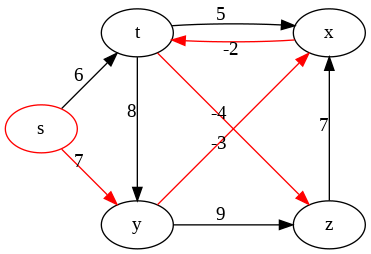
\includegraphics[width=0.99\columnwidth]{fig/shortest_path_trees_0.png}
    \caption{$s$ as source}
    \end{subfigure}
    \begin{subfigure}{.32\textwidth}
    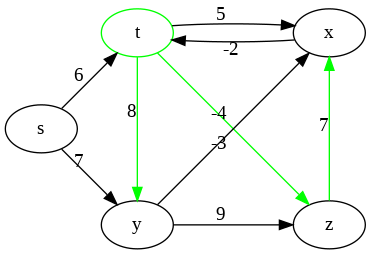
\includegraphics[width=0.99\columnwidth]{fig/shortest_path_trees_1.png}
    \caption{$t$ as source}
    \end{subfigure}
    \begin{subfigure}{.32\textwidth}
    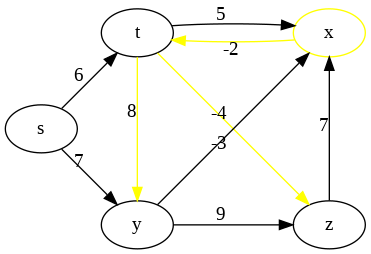
\includegraphics[width=0.99\columnwidth]{fig/shortest_path_trees_2.png}
    \caption{$x$ as source}
    \end{subfigure}
    

    \begin{subfigure}{.32\textwidth}
    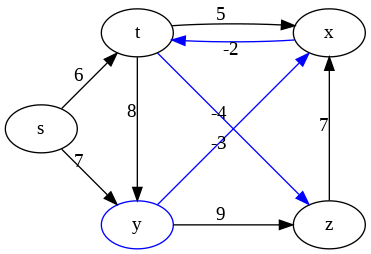
\includegraphics[width=0.99\columnwidth]{fig/shortest_path_trees_3.png}
    \caption{$y$ as source}
    \end{subfigure}
    \begin{subfigure}{.32\textwidth}
    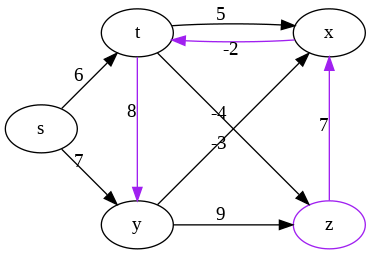
\includegraphics[width=0.99\columnwidth]{fig/shortest_path_trees_4.png}
    \caption{$z$ as source}
    \end{subfigure}
    \caption{All shortest-path trees starting from each vertex.}
    \label{fig:shortest_path_tree_all}
\end{figure}
We reconstruct the shortest-path trees and visualize them in Fig.~\ref{fig:shortest_path_tree_all}. 
% \paragraph{What will learn?}
% Just as in previous section the predecessor subgraph $G_\pi$ forms a shortest-paths tree from a given source vertex, the subgraph induced by the $i$-th row of the $\Pi$ matrix should be a shortest-paths tree with root $i$. 
% The standard All Pair Shortest Path algorithms such as matrix multiplication like shortest paths algorithm and Floyd–Warshall algorithm are just like Bellman–Ford, and are also application of Dynamic Programming.
% For $n$ nodes in a graph, if there exists no negative-weight cycles, then for every pair of vertices there is a shortest path that is simple and thus contains at most $n-1$ paths. Therefore, we end up having $\sigma(i,j)=l^{(n-1)}_{ij}=l^{(n)}_{ij}=l^{(n+1)}_{ij}$. 
\subsubsection{Repeated Squaring Extended Bellman-Ford Algorithm}
We leverage the second DP approach in Section ~\ref{chapter_advanced_graph_sec_algorithm_design}. This approach bears resemblance to the repeated squaring optimization in matrix multiplication. % in the case of with extra outer loop over $|V|$ vertices as source vertex. The benefits from being matrix multiplication like is we can further improve its efficiency using matrix multiplication optimization which is called \textbf{Repeated Squaring}.  
Repeated squaring is a general method for fast computation of exponentiation with large powers of a number or more generally of a polynomial or a square matrix.  The underlying algorithm design methodogy is divide and conquer. Assume our input is $x^{n}$, where $x$ is an expression, repeat squaring computes this in $O(\log n)$ steps by repeatedly squaring an intermediate result. Repeating Squaring method is actually used a lot in some advanced algorithm. Another one we will see in String algorithms. 
\paragraph{Repeated Squaring Applied on Extended Bellman-Ford Algorithm}
If we observe the \texttt{bellman\_ford\_one\_pass}, it has three for loops, and it shows similar pattern with matrix multiplication. Suppose $A$ and $B$ are both $n\times n$ matrix, and we compute $C=A\times B$, the formulation is $c_{ij} = \sum_{k=0}^{n-1} a_{ik}\cdot b_{kj}$ which has the same pattern as of Eq.~\ref{eq_recurrence_extended_bellman}.  If we use $\cdot$ to mark \texttt{bellman\_ford\_one\_pass} operation on $L$ and $W$, we will have the following relations:
\begin{align}
    L^{1} &= L^{0}\cdot W = W,\\\nonumber
    L^{2 }&= L^{1}\cdot W = W^2, \\\nonumber
    L^{3 }&= L^{2}\cdot W = W^3, \\\nonumber
     &\vdots\\\nonumber
     L^{n-1 }&= L^{n-2}\cdot W = W^{n-1}\nonumber
\end{align}


With repeated squaring technique, we can compute $L^{n-1}$ with only $\log (n-1)$ round of one pass operation
\begin{align}
    L^{1} &= W,\\\nonumber
    L^{2 }&= W \cdot W, \\\nonumber
    L^{4 }&= W^2 \cdot W^2, \\\nonumber
     &\vdots\nonumber
\end{align}
The above repeation stops when our $m \geq n-1$. The implementation is:
\begin{lstlisting}[language=Python]
import copy
import math
def bellman_ford_repeated_square(L):
  n = len(W)
  for i in range(n): # source
    for j in range(n): # endpoint
      for k in range(n): # double the extending length
        L[i][j] = min(L[i][j], L[i][k]+L[k][j])
  
def extended_bellman_ford_repeated_square(W):
  n = len(W)
  # initialize L, first pass
  L = copy.deepcopy(W)
  print(f'L1 : {L} \n')
  # log n passes
  for i in range(math.ceil(math.log(n))):
    bellman_ford_repeated_square(L)
    print(f'L{2^(i+1)}: {L} \n')
  return L
\end{lstlisting}

\subsubsection{The Floyd-Warshall Algorithm}
We leverage the third DP approach in Section ~\ref{chapter_advanced_graph_sec_algorithm_design}, this approach is called \textit{The Floyd-Warshall Algorithm}. We directly put the code here:
\begin{lstlisting}[language=Python]
def floyd_warshall(W):
  L = copy.deepcopy(W) #L0
  n = len(W)
  for k in range(n): # intermediate node
    for i in range(n): # start node
      for j in range(n): # end node
        L[k][i] = min(L[k][i], L[k][j] + L[j][i])
  return L
\end{lstlisting}
\end{document}